%
%  Author: P.N. van Kempen
%

%\pdfcompresslevel=0		%  speedup pdf creation, disable for final version
%\pdfobjcompresslevel=0	%  speedup pdf creation, disable for final version
\documentclass[a4paper,oneside]{memoir}


%
%  Configuration
%
\newcommand{\shortdoctitle}{Master's Thesis}
\newcommand{\doctitle}{Option Valuation in the Aviation Industry}
\newcommand{\me}{P.N. van Kempen}
\newcommand{\keywords}{Options, Airfare lock-in, tickets}
\date{\today}	%  \today or yy-mm-dd

%\newcommand{\biblioname}{ThesisBiblio}	%  insert name of bibliography (without .bib)


%
%  Packages
%
\usepackage[T1]{fontenc}
%\usepackage{charter}					%  non-standard font
\usepackage{tgpagella}					%  or use this font

\linespread{1.15}

%\usepackage[expert]{mathdesign}		%  normal style for equations (necessary?)

\usepackage{amsmath, amsfonts, amssymb}
\usepackage{kbordermatrix}

\usepackage{booktabs}				%  better looking tables
\usepackage{multirow}
\usepackage{longtable}
\usepackage{xcolor}					%  colors!!
\usepackage{flafter}				%  show figures, etc. only after appearance in text
\usepackage{graphicx, pgfplots}	    %  figures and plots
\usepackage{subfig}                 %  figures side-by-side
\usepackage{marginnote}				%  notes in margin
\usepackage{microtype}				%  better formatting
\usepackage{paralist}				%  list control
\usepackage{titlesec}				%  chapter header style

\usepackage{pdflscape}


\usepackage{tikz}					%  drawing
\usetikzlibrary{trees,shapes,arrows}

\usepackage[hidelinks]{hyperref}	%  crosslinks without ugly surrounding box
\usepackage{cleveref, nameref}		%  link to labels by actual names
\usepackage{apacite}				%  apa style bibliography

%
%  Definitions
%
\author{\me}
\title{\doctitle}


%own chapter style
\titleformat{\chapter}[display]
	{\centering\bfseries}
	{\Large\thechapter}
	{.8ex}
	{\titlerule \vskip 0.8ex \huge}

%insert .tex figures. \insertfigure{<filename> (must be in figures/)}{<caption>}
%this also creates label 'fig:<filename>'
\newcommand{\insertfigure}[2]{
\begin{figure}
	\center
	\input{figures/#1}
	\caption{#2}
	\label{fig:#1}
\end{figure}
}

%  generate link with type and name of #1 (e.g., 'chapter Introduction')
\newcommand{\typenameref}[1]{\namecref{#1} \emph{\nameref{#1}}}

%  generate todo. \todo[<inplace text> (default is 'here')]{<margintext>}
\newcommand{\todo}[2][here]{{\color{red} #1\marginnote{#2}}}


%  for assumptions
\newcounter{assumptions}
\newcommand{\assumption}[1]{%
    \stepcounter{assumptions}%
    \begin{quote}\emph{Assumption \theassumptions: #1}\end{quote}%
}

%  for parameters
\newcounter{parameters}
\newcommand{\parameter}[1]{%
    \stepcounter{parameters}%
    \begin{quote}\emph{Parameter \theparameters: #1}\end{quote}%
}

%  scientific notation
\providecommand{\e}[1]{\ensuremath{\times 10^{#1}}}


%
% PDF settings
%
\hypersetup{
    pdfauthor={\me},
    pdftitle={\shortdoctitle},
    pdfsubject={\doctitle},
    pdfkeywords={\keywords}
}


\sloppybottom	%  prevent orphan/widow lines
\begin{document}
%  Frontmatter
\frontmatter
%{\linespread{1} \begin{titlingpage}
\begin{center}
\large

\vspace*{1.5cm}

\includegraphics[width=0.32\textwidth]{figures/EURlogo.pdf} \\[0.7\baselineskip]
\textsc{\Large erasmus university rotterdam\\
		msc supply chain management} \\[1.5\baselineskip]
 
\rule{\textwidth}{1.2pt}\vspace{-\baselineskip}\vspace{1.8pt}
\rule{\textwidth}{0.4pt} \\[2.6\baselineskip]

\textbf{\LARGE AIRFARE LOCK-IN PRODUCTS} \\[1.0\baselineskip]
\textsc{\Large Option Valuation in the Aviation Industry}\\[1.8\baselineskip]

\rule{\textwidth}{0.4pt}\vspace{-\baselineskip}\vspace{2.4pt}
\rule{\textwidth}{1.2pt} \\[2.25\baselineskip]

\textsc{Rotterdam, \today} \\[3.75\baselineskip]

\begin{minipage}[b]{0.4\textwidth}
	\flushleft
	\textsl{Author} \\[0.1\baselineskip]
	P.N. van Kempen \\
	322165
	\vfill
\end{minipage}
\begin{minipage}{0.4\textwidth}
	\flushright
	\textsl{Supervisor} \\[0.1\baselineskip]
	dr.~ir.~N.A.H. Agatz \\[1.2\baselineskip]

	\textsl{Advisor} \\[0.1\baselineskip]
	dr.~N. Mishra
\end{minipage}


\end{center}
\end{titlingpage}
}
%\renewcommand*\abstractname{Executive summary}
\begin{abstract}
Airlines have to operate on low profit margins while dealing with extreme risks and uncertain demand. To cope with these challenges, the aviation industry has implemented revenue management models. The models allowed companies to better segment their customers and make more accurate estimates of a passenger's maximum willingness to pay. While this has led to large increases in revenues for the airliners, customers have to deal with much higher levels of uncertainty. Airfares might jump hundreds of dollars overnight, and insuring yourself for possible cancellation is many times more expensive than the cheapest airfare.

In this master's thesis, I want to study the concept of \emph{airfare~lock-in products} and test whether it is viable for an external company without capacity information to sell this new type of goods. Airfare~lock-in products allow the customer to fixate the price of a seat for a predetermined period at a certain premium. The customer can thus decide at a later moment in time whether to actually buy the ticket or not, while covering himself from price increases. Furthermore, when an airfare drops a large amount, the customer can still choose to not execute the product and buy the ticket at the lower rate. An airfare~lock-in product therefore also allows the customer to gain from price decreases. This concept is thus comparable to call options in financial markets.

I will research the viability of offering such options by training and testing historical data. Data on 22~routes is collected for flights departing in a period from August $19^{th}$ till September $30^{th}$. Each flight's fare is checked 4~times per day for a period of 6~weeks before departure. The first 4~weeks of the census (i.e., August $19^{th}$ -- September $16^{th}$) will be used to train two option valuation models. The first method will base its predictions using the Black--Scholes method, while the other approximates the best option price using Monte Carlo. After the creation of the models a simulation will be run based upon the last two weeks of the historical data. This simulation tests the profitability of the two models and compares them with the most optimal situation. It will analyse whether it is theoretically and practically possible for an external company that sells the options to sustain. Furthermore, the simulation will also conclude which of the option valuation models approximates the optimal option price best.

After the simulation a sensitivity analysis will be performed as well. In this analysis the three~parameters of a passenger --- \begin{inparaenum}[\itshape (i)\upshape]
\item risk-utility,
\item forecasting technique, and
\item likelihood of travelling
\end{inparaenum} --- will be altered to see what the effect of these properties is on the profitability of the company that offers airfare~lock-in products.


\todo{update}
\end{abstract}

\newpage

\begin{Spacing}{1.4}
	\small
	\tableofcontents
	\newpage
	\listoffigures
	\listoftables
\end{Spacing}

%%  Mainmatter
\mainmatter
\chapter{Introduction}
\label{chap:Introduction}
\chapterprecishere{The fastest way to become a millionaire is to start off with a billion dollars and invest in an airline}

It might not come as a surprise that companies in the aviation sector have to operate on profit margins close to none\footnote{\url{http://on.wsj.com/MftvqH}}, and that they were struck hard by the financial crisis. To cope with these challenges, airliners are known to implement many revenue management concepts (e.g., market segmentation, protection levels). Robert Crandall, former CEO of American Airlines, even said stated that yield management is ``\emph{the single most important technical development in transportation management since we entered deregulation}'' \cite[p.~30]{cross97}.

The implementation of such revenue management models has caused major changes in the aviation sector. For instance, the application of booking protection levels has created many fluctuations in airfares within a single flight. Early bookers usually can purchase a ticket at a low rate while passengers later in the booking process can only acquire the same seat at a much higher fare. Early booking of a flight, however, brings along much more uncertainty, as there might occur many situations in which the buyer is unable to utilize the ticket. For example, when a passenger wants to go skiing, but breaks his leg prior to departure. A person can cover himself from any losses caused by these kind of situations by buying insurance. However, insurance does not always provide a solution for no-shows. By way of illustration, consider you would like to go on holiday with a group of your friends, but your friends are undecided over whether they can go on the trip or not. Now you have two options to choose from:
\begin{compactitem}
    \item buy the flight now and risk not using this ticket because your friends can't come along, or
    \item wait to buy the flight until you know for sure your friends will go and risk sudden price increases in airfare or even sell-outs.
\end{compactitem}
\noindent
This extra level of uncertainty is undesired for customers, and makes it more difficult to let them make rational decisions.

A recent trend in the aviation industry might provide a solution to this problem of uncertainty. Airliners offering \emph{airfare~lock-in products} allow their customers to cover themselves for certain risks. An airfare~lock-in product allows a customer who is unsure whether he wants to directly buy a ticket to buy an \emph{option} on that flight instead. The option gives her the opportunity to buy the actual ticket at a later time at a predetermined price. Some airliners (e.g., United Airlines, Air France-KLM, Estonian Air) already offer this new type of service and allow the customer to reserve a seat for 2~to 14~days. New external companies like OptionIt, options away, SteadyFare, also arise, though all still in their initial stage\footnote{OptionIt currently offers only options for sporting events, but plans to offer options for tickets of major airlines. The company options away just made their service available to the public, and SteadyFare is not available for public use}.

The offering of lock-in products might be valuable to passengers and external companies that write these options, as well as the actual airlines. However, research on this topic is scarce and results of successful applications of the strategy are not yet public. Further theoretical and empirical research might provide answers to the actual viability, and could offer support for companies that would like to implement this type of product.

\subsection{Research objective and questions}
In this thesis I would like to contribute to the topic of options in the aviation industry. I will do so by studying whether external companies can offer these kind of airfare~lock-in products in a sustainable way. Furthermore, I want to test different option valuation models, and see under which conditions the model performs best.

This research could therefore be useful to companies that write such options, as well the airline carrier of the underlying flights. On a more general perspective, concepts studied in this thesis might also be applicable to other organizations that have to deal with perishable services. Think of other travel-related companies like hotels or car-rental services, or in industries where uncertainty might withhold consumers to buy products like ticket sales for basketball games. This Master's thesis could offer insights into these kinds of industries as well.

The first main research question that I will try to provide an answer to can be defined as follows:

\begin{quote}\emph{Is it sustainable for an external company without capacity information or seat reservation capabilities to set the price of airfare~lock-in~products at a level that the customer accepts?}\end{quote}

As \autoref{chap:Results} will show, a company could operate in a viable way by relying on selling airfare~lock-in products. While the theoretical model reveals that profits in a risk neutral setting with an all knowing customer are not possible, a more realistic scenario with an inaccurate customer does lead to positive outcomes. The simulation with a seller making predictions using a very practically implementable forecasting method --- Monte~Carlo simulation --- even shows that positive results could be realized.

The second question I will research in my thesis, is associated with the benefits an option offers to the customer:

\begin{quote}\emph{What are the implications for the customer resulted from the purchase of an an airfare~lock-in product?}\end{quote}

As will be shown in \autoref{subsec:CustomersAdvantages}, the purchase of an option on a flight ticket might be beneficial to the customer in certain situations. When the customer makes more inaccurate price movement predictions relative to the seller, he will more likely make the wrong initial decision, and is thus better off buying the lock-in product. A higher inaccuracy of the passenger results in higher expected cost savings when buying te option.

For the third and final research question in my Master's thesis, I will study the effects of different characteristics of the option seller and customer to determine their influence on the optimization of the company's profits. These characters include \emph{company's level of forecasting accuracy} (i.e., how accurate are the seller's predictions of future price movements), \emph{company's level of applied margin} (i.e., how much does the seller add to the option price to gain profits and account for forecasting inaccuracies), and the \emph{customer's level of forecasting accuracy}:

\begin{quote}\emph{What are the effects of the option seller's level of forecasting accuracy and applied margin, and the customer's level of accuracy on the performance of the model?}\end{quote}

The simulation models run in \autoref{chap:Results} will reveal that these factors play a significant role in the performance of the model. For example, the analysis showed that the applied margin offers the option selling company a good technique to compensate for higher forecasting inaccuracies, and will a lower prediction accuracy of the customer result in more benefits for her when buying an option.


\subsection{Scope of research}
This study will analyse a set of 22~different single-legged routes covering flights within the United States and Europe, as well as intercontinental legs (see \autoref{app:SelectedRoutes} for a the selected routes). Results of this research will therefore be generalizable to flights falling within the boundaries of this particular set. As being stated previously, the findings might also be applicable to industries where similar perishable services are being offered.

Furthermore, this research will build its models based upon theoretical frameworks and empirical data that is available to the public. I will thus consider the third party as an independent option writer that does not have any inside information or capabilities other than a customer has. For instance, the model will assume that the external company has no possibility of reserving capacity on a flight, and therefore has to deal with the risk of sell-outs. In a practical situation, however, the company might make an arrangement with the operating carrier to reserve seats for a certain premium. This would cut uncertainty for the option writer, and thus decrease option prices. The model I use in this study might therefore be harsher than realistically would be the case.


\subsection{Methodology}
To provide answers to the proposed research questions, I will collect pricing data on a select number of flights for a period of six~weeks. After the collection and parsing of these data, I will run several simulations on this empirical information to see under what conditions the model might be viable.

The first model will assume an all knowing seller which has perfect information on the buyer, and can make predictions with $100\,\%$ accuracy. This model will be used as a benchmark to compare the more realistic models with, and will offer insights in the influence of certain characteristics as formulated in research question three. Later models will release the assumption of the all knowing seller, and assume a seller that uses strong-form rational expectations and Monte~Carlo simulation to make its price movement predictions. The customer will either also make use of strong-form rational expectations, or base her predictions on the weak-form case.



\chapter{Literature Review}
\label{chap:LiteratureReview}
\section{Yield management in the aviation industry}
According to \citeA[pp. 2]{anderson2004revenue} the term yield management can be described as ``\textit{[the] process of managing perishable inventories to maximize the total revenue from these inventories}''. The aviation sector was the first industry to apply this concept of revenue management. The costs of the services airlines sells are mostly fixed (e.g., fuel, maintenance) and consist  of negligible variable costs (e.g., meals) \cite{o2001introduction}. In such a scenario, unsold seats become obsolete upon departure and would result in lost revenues to the company. A more airline-related definition of yield management is given by \citeA[pp. 136]{akgunduz2007using}, who state that ``\textit{revenue management is [\ldots] the practice of managing the booking requests with an objective of increasing the sales revenues}''.

\citeA{smith1992yield} defined three major changes in the aviation industry which contributed to the development of yield management. These changes, which all occurred in the 1960's and 1970's, had to do with:

\begin{description}
\item[Deregulation]
Arguably the most important factor in the creation of revenue management in the aviation industry is its deregulation. The deregulation was formed by the approval of the \citeA{airlinederegact}, and removed price, route and entry restrictions on airlines. After removal of these restrictions, airliners were allowed to set their own prices. The ability to change prices for different segments of customers is one of the core concepts of revenue management.

\item[Automated reservation systems]
Computerized reservation systems allowed airlines to centrally control reservation activity, and process and store huge amounts of data. With the development and implementation of the Semi-Automated Business Research Environment (SABRE) in 1966, American Airlines pioneered in the field of online reservation systems for the travel industry \cite{voneche2005yield}. The data acquired via the system could be analysed and used to forecast the booking process, and automatically adjust airfares of flights according to their demand.

\item[Discount fares]
The idea behind the concept of discount fares is to offer reduced prices to specific segments of customers to sell seats which would otherwise be empty \cite{belobaba1987survey}. This concept added a whole new dimension to the airline industry. For instance, by offering low prices to low-grossing customers early in the booking process, there would be fewer seats to sell to high-grossing travellers. The concept of determining the right amount of tickets with discount at specific times is called \emph{Discount allocation}.
\end{description}

Discount allocation has its origin in the article by \citeA{littlewood1972forecasting}. In his paper, for which he would receive the \citeA{informs13} in 2004, Littlewood described a number of approaches to handle the allocation of discount fares in the airline industry. By predicting future demand and analysing consumer sell-up behaviour, one would be able to create a better allocation of price discounts which resulted in a higher load factor and revenues for the airlines. More specifically, Littlewood's rule states that a ``\textit{request for a seat should be fulfilled only if its revenue exceeds the expected future value of the seat in question}'' \cite[pp. 17]{wright2010dynamic}.

For the concept of discount allocation, historical pricing and demand acquired by the implementation of computerized reservation systems proved to be very useful to create more accurate predictions \cite{littlewood1972forecasting}.

In their paper, \citeA{smith1992yield} describe the case of revenue management at American Airlines. Of all the airliners, American Airlines was the first to actually implement the theory of yield management in the 1970s. After years of research in the 1960s, the company developed an application using the data acquired via their computerized reservation system, SABRE. The system, which was later named DINAMO, was based upon the concepts described by \citeA{littlewood1972forecasting}, and implemented the options of overbooking, discount allocation and traffic management \footnote{traffic management is the optimal reservation of single-legged flights to provide for higher-profit multi-legged flights, while preventing empty seats}. The system decreased the spoilage of unsold seats from 15~percent to 3~percent \cite{smith1992yield}. Furthermore, in 1992, the former CEO of American Airlines, Robert Crandall, showed that yield management contributed to an increase of \$~1.4 billion in revenues and an estimated \$~500 million of extra profits in the first three years after implementation of DINAMO.

While the introduction of discount fares increased utilization of aircrafts and significant expanded revenues of airliners, it also resulted in higher uncertainty for consumers. Where the customers first could base their decisions on linear prices, airfares have become very dynamic and follow unintuitive paths. As an example, \citeA{groves2013agent} state in their paper that, in contrast to popular believe, the principle to buy tickets early in the booking process to avoid an increase in price is suboptimal. Their research shows that this strategy almost always results in higher prices and could be easily outperformed by other models (see \label{subsubsec:PredictabilityOfAirfares} for a complete description of their article).

To overcome the problem of uncertainty created by yield management, new theories of pricing have been developed. One such example is the theory of \emph{real options} as described by \citeA{amram1999real}. These specific kind of options use the framework developed by modern financial instruments to cope with uncertainty of underlying assets. In accordance, \citeA{dixit1996investment} argue that in the presence of uncertainty and managerial flexibility in operating strategies, real option may provide a solution.

The practice of yield management is not only restricted to the aviation industry, but applies to many other sectors. \citeA{kimes1989yield} supplies a list containing common characteristics of industries that successfully applied revenue management:
\begin{compactitem}
\item relatively fixed capacity;
\item ability to segment markets;
\item perishable inventory;
\item products sold in advance;
\item fluctuating demand;
\item low marginal sales cost/high marginal capacity change cost.
\vspace{1ex}
\end{compactitem}

\citeA{harris1995hold} give in their paper a few examples of industries that all share these characteristics, namely: hotels, car rental agencies, railroads, cruise ships, printing and publishing. Dynamic pricing due to revenue management practices creates uncertainty on the customer-side in these sectors as well. So, the theory of real options could also be applied to these industries.

In the next section I will analyse current research on this topic and give an over\-view of option-based models applied to these kind of industries.

\section{Real options in current industries}
An option gives its holder the right, not the obligation, to buy or sell (respectively named \emph{call}- and \emph{put}-options) a specific underlying asset on or before a certain date (\emph{maturity}) for a predetermined price (\emph{strike price}) \cite{hull99}. A real option differs from a financial option, in that the underlying asset is a tangible object, rather than a derivative. Furthermore, real options are not normally not tradable like financial options are. Therefore they are often referred to as \emph{deferral options} \cite{jain11}.

A real option is most commonly used as an alternative to the \emph{net present value}-method for managing capital budgeting. However, this type of could also be applied to set up contracts for other tangible assets. This last category of options can be offered to consumers to sell for example tickets for games, energy or insurance. In their paper, \citeA{sainam2010consumer} provide another type of option even more consumer related. The option, for which they coined the term \emph{consumer option}, is like a real option, but the quality of the outcome is different per consumer segment. The authors give the example of the final of a sports tournament, where a customer only wants to see the final when his team is playing. When the customer's team did not make the finals, he or she will not exercise the option.

The term \emph{consumer option} is not often used in literature, and authors usually use \emph{real options} to also refer to consumer options. To avoid confusion, I will use the term \emph{real option} to refer to all options with tangible underlying assets which are provided to consumers.

An important distinction between options is the time at which holders are allowed to execute the contract \cite{hull99}. On the one extreme, there are \emph{European} options, which allow the customer to only execute its option \emph{on} the specified maturity date. At the other end of the spectrum are \emph{American} options, which allow the holder to execute their right \emph{before} the determined maturity date. In between these two types of options there are many alternatives, like Bermudan or switch options which allow execution of options a certain number of times before maturity date. An example implementation of such an option can be found in utility markets.

\subsection{Utility industry}
An industry in which a real-option model is already applied, is the utility industry \cite{keppo2004pricing}. The options, called \emph{swing options}, are traded over-the-counter by energy suppliers to their customers. A consumer buys a forward contract which obliges him to buy a predetermined amount of electricity for a certain period at a specific price. To allow for flexibility, a customer can bundle this forward contract together with the swing part, which gives him the right to change the amount a number of times during this period \cite{jaillet2004valuation}. The swing option thus gives the holder the opportunity to have a set price, while he is still able to respond to uncertainty by changing the amount of energy when circumstances change.

\citeA{thompson1995valuation} was the first researcher to determine the optimal price of such a swing option. He created a tree-based path-dependent  model based upon previous research by \citeA{hull1990valuing}, and used dynamic programming to numerically approximate the best value of these contracts. The author admits that solving path-dependent is difficult, because - in the case of swing options - prior exercise decisions influence the outcome of the model. This makes it very hard to determine the optimal price of the swing option analytically.

\citeA{jaillet2004valuation} present in their paper a valuation framework for swing options. The authors based their model on multilayered trinomal trees. The concept of trinominal trees for the use of option valuation was first used by \citeA{boyle1986option}, and allows to evaluate the contract on multiple decision variables. \citeA{jaillet2004valuation} also state in their paper that exact valuation of options in path-dependent models is difficult, and their proposed model faces the same difficulties as in other real option frameworks.

Both of the previously described techniques use numerical techniques that use trees to evaluate the optimal price of a swing contract as a whole. \cite{keppo2004pricing} on the other hand, replicates the swing contact by a future contract and a call option. The author estimates price the call part by looking at the commodity exchange market by using the Black--Scholes method \cite{black1976pricing}. He also concludes that due to the swing option's path dependency and Bermudan style, it is not possible to solve the problem algebraically.

Swing options have some similarities with airfare lock-in products, but there are also large differences. For example, costs when switching from energy providers are high and often impossible due to contracts. Customers are `stuck' at their current energy provider, while in the airline industry, one can easily switch between airliners without additional costs. Furthermore, a swing option can be seen as multiple European and/or American options, which creates path dependency. Options for airline tickets consist of a single European or American option. Lastly, \citeA{jaillet2004valuation} state that the uncertainty of a swing option is determined by the unpredictability of prices (future part) combined with the quantity which is actually needed (swing part). The uncertainty of airline tickets, however, is primarily based upon the unpredictability of prices.

\subsection{Car rental industry}
Car rental agencies continuously face the problem of allowing a vehicle to be booked for a future time right now, or rather wait and sell the car at a higher rate in the future. When the agency decides to rent out the car right now there might be missed revenues due to not being able to offer high-end customers a product. On the other hand, when agencies refuse the current booking, they face the probability that the car is not booked at all. This would result in even higher loss of revenues as the car has `perished' and can never be rented out for that passed date again. According to \citeA{anderson2004revenue}, this classic revenue management problem is similar to the swing option method described in previous section. They present the case of real options applied to the car rental industry by trying to apply the swing option model currently available in electricity and gas industries to the operating agent of such a company. In the paper the authors were able to solve the operator's optimal rental strategy by considering the operator as the holder of a swing option on car rentals.

While \citeA{anderson2004revenue} state in their article to have found an optimal solution to this problem which is extendible to other industries, they also indicate some difference among the car rental and airline industry.

First, the authors state that airliners offer airfares by opening and closing discrete pricing classes. While the car rental industry also has different classes (size, AC, \ldots), they also differ prices within each class. This form of dynamic pricing is more difficult to predict, and hence creates more uncertainty. Secondly, car rental customers are less prone to changes in fares, while this is not the case in the airliner industry. And lastly, this model might not be applicable to this research as it defines the concept the other way around. The framework presents the idea in which the operators use swing-like options to determine the best car rental strategy. However, this paper focusses on the ability of \emph{customers} to buy real options to lock in airfares.

\subsection{Tournament industry}
A more recent adoption of real options handling uncertainty, is the category associated with the sports market. Tickets for games usually sell weeks before the actual game. Fans of a team are willing to pay a large sum for a ticket when their team actually plays in the finals, but less or even nothing when this is not the case. However, the outcome of the actual teams that play in the finals is often not known in advance. Furthermore, customers need to buy tickets early in advance to prevent sell-outs. This puts the fans at risk, because there is a probability that their favourite team does not play in the finals. According to \citeA{sainam2010consumer}, this uncertainty creates a suboptimal situation where ticket agencies cannot charge the best prices due to customers taking into account the possibility that they buy a ticket for a final in which their favourite team does not play. The authors propose a new concept in which, instead of the ticket, customers buy real options. This real option gives its holder the right to buy the actual ticket when the outcomes are known.

To test this concept, \citeA{sainam2010consumer} empirically compare three pricing mechanisms, knowing:
\begin{description}
\item[Selling in advance] This is the current situation. Customers buy tickets well in advance and hope that their team plays the actual finals;
\item[Pricing on full information] Customers are sold tickets after the outcome of teams in the final is known;
\item[Providing real options] In this concept the customer first buys an option well in advance which gives him the right to attend the game. When the outcome is known, the customer can decide whether to exercise the option for an extra amount.
\end{description}

The authors studied the concept using these three pricing mechanisms, and showed that in many cases revenues where higher when applying the \emph{real options}-model, rather than \emph{advance} or \emph{full information} selling.  This was due to the fact that agencies can charge higher prices, because the \emph{willingness to pay} of customers is not driven down by uncertainty. The concept also generates extra revenue from selling real options, and expands the existing market due to customers willing to buy tickets at a low rate of uncertainty. The profit advantage for option selling was highest when uncertainty was highest, which clarifies the purpose of options. The paper also found that \emph{risk-averse} customers are willing to pay more for their ticket under uncertainty than their \emph{non-risk averse} counterpart.

\citeA{berkowitz2012real} even go further into this concept and propose a concept in which customers can \emph{only} exercise their options when their favourite team reach\-es a given round. Furthermore, the authors suggest that a combination of advanced selling and real options might increase a ticket agency's revenue even further due to segmentation of game- and team-based fans. In their paper, the authors test this proposition and come to the conclusion that not only the revenue increases for the organizer, but also the utility of fans due to the fact that they are sure to have a ticket when their team plays in the finals. Lastly, more fans from the playing teams are present, which could increase the experience of the spectators.

\citeA{balseiro2011revenue}, who apply a combination of the models proposed by \citeA{berkowitz2012real} and \citeA{sainam2010consumer}, also show these increases in revenue. They argue that this is due to the ability to better segment customers and thus better determine their \emph{willingness to pay}. Furthermore, they argue that the extra certainty increased social welfare of the customer.

\citeA{berkowitz2012real} state in their paper that their model could be used in many other industries as well. The authors give examples of which airline tickets is amongst them. While similarities can be found on a very abstract level (like the \emph{binary option approach}), there seem to be major differences among the industries. For example, finals for sport events have close to no fluctuations in price and a very high sell-out probability closer to the date of the final. In the aviation industry, however, high fluctuation in price is much more common. Furthermore, flights do sell-out, but often this is not the case \footnote{currently the average load factor is 83.6~percent. See \url{http://www.transtats.bts.gov/}}. Also, the few number of alternatives in sporting events creates less price elasticity of customers. This is not applied to the aviation sector where a small change in price might cause a customer to switch to another vendor.

\subsection{Aviation industry}
\label{subsec:AviationIndustry}
The first occurrence of option pricing in the aviation industry in literature is provided by \citeA{walker1998method}. In their patent, the authors provide a system which determines the price of an option on a specific flight. This option gives the holder the right to buy the ticket at a moment in the future at the specified price, without actually holding the risk of sell-outs and increases in airfares. According to the authors, real options sold in this kind of setting have three major differences compared to traditional financial options:
\begin{compactenum}
\item the product is only supplied by a number of airlines;
\item the product is not interchangeable, because customer might only want to fly with a specific airline at a specific time and date;
\item there are only a finite number of seats available (capacity constrained).
\vskip 1ex
\end{compactenum}

To overcome these differences, they describe a system which evaluates options with a method other than the traditional systems. The method determines the price of an option by multiplying a base price for the option by several relevant factors. These factors include: \emph{number of days before departure}, \emph{expected load of aircraft}, \emph{desirability of the customer} (low-grossing versus high-grossing), \emph{flexibility of the customer's flight plans}, and \emph{historic volatility of ticket prices}. 

\citeA{jain11} argue in their paper that traditional option valuation methods like the \emph{Black--Scholes} model \cite{black1976pricing} can actually be applied to this type of real options. The followed prices of 14~flights for 79~days during a period from November~2005 till February~2006. After collection of the data, the authors used the Black--Scholes model to evaluate the theoretically best price for a call- and put-option with a maturity date of 79~days (i.e., ticket bought on 79~day before departure) on these specific flights. The authors calculated the affordability of each option, which they defined as price of an option divided by the average ticket price of the flight ($p_o/\bar{p_f}$). Their results show that the affordability of lock-in~products on their analysed flight range from 2.46~percent to 11.28~percent. The average affordability across all 14~flights is 7.2~percent. Put options to lock-in the price range from 1.55 to 10.34 with a mean of 6.37~percent of the ticket's price.

One major limitation according to \citeA{jain11}, is that their analysis is based on \emph{ex post data}. This means that the option price, including the volatility, was based upon data that was only available to the customer in the future. While the authors recognize this as a major flaw in their research, they argue that this data is available at the airliners.

Other types of real options are more prevalent in the aviation industry. For example, \citeA{akgunduz2007using}, \citeA{gallego2008revenue}, \citeA{ching2010improving}, all describe the use of options in the booking process of an airliner. They illustrate the concept in which airliners sell tickets with a very high discount to customers early in the booking process. Coupled with these low-fare tickets the airliner buys a call option, which gives them the right to recall the ticket when capacity is needed for higher-grossing customers. This gives the airliner the opportunity to sell tickets at high-fares when demand is high, while still having the backup of the low-fare customer to prevent empty seats. A put option is also described, in which a travel agent agrees upon buying tickets from the airline at a very low-fare when these are still available close before departure of the flight. This allows the airliner to still sell tickets which would have been empty seats otherwise.

The previously mentioned authors all use numerical methods to determine the optimal mix of call/put and normal seats. Their shared conclusion is that this type of yield management is superior to the current overbooking methods, because it generates more revenues and also higher social welfare for customers. The model is also applicable to other concepts. \citeA{graf2011option} and \citeA{graf2013transfer} show for example that this concept of capacity based option pricing can be implemented at airline alliances. In this situation, the operating airline can sell options to the ticketing airline. When the ticketing party sells a seat of higher value than the strike price of the option, it exercises the option. The operating carrier can also buy a put option on the sold call option. These kind of option on options, also defined as \emph{compound options} \cite{trigeorgis1996real}, give the operator the right to recall options from the ticketing company when demand is high. In a strategic alliance this only happens when the revenue gained from accepting a seat request is greater than the strike price plus the option price \citeA{graf2011option}. The authors use simulation-based evaluation of booking limits (i.e., how many calls and puts to sell) to determine the best scenario of such an options.

\section{Option valuation methods}
\subsection{Theoretical model: Black--Scholes}
The most used options valuation method for pricing options in financial markets is the Black--Scholes model \cite{hull99}.  It was first proposed in a paper by \citeA{black1973pricing}, and was later expanded mathematically by \citeA{merton1973theory}. The model calculates the value of an option for the underlying stock. The article shows that the expected rate of return of the underlying asset and risk preference of the investor do not matter. The formula rather uses other variables (e.g., volatility of the underlying asset, maturity, risk-return rate) to estimate the theoretical option price. The Black--Scholes formula is defined as follows:
\begin{align*}
C(S, t) &= N(d_1)S - N(d_2) Ke^{-r(T)} \\
d_1 &= \frac{\ln(S/K) + (r + \sigma^2/2)(T - t)}{\sigma \sqrt{T - t}} \\
d_2 &= d_1 - \sigma \sqrt{T - t}
\end{align*}

\noindent
\citeA{black1973pricing} make a few assumptions of the underlying stock, including:
\begin{compactitem}
\item The option style is European;
\item The stock price follows a geometric Brownian motion (i.e., log-normal distribution) with constant drift and volatility;
\item The stock pays no intermediary dividends.
\end{compactitem}

\noindent
These assumptions might also be applicable to airfares. For instance, a rational customer would only exercise its airfare~lock-in product at maturity (see \typenameref{sec:OptionStyle} in \cref{chap:Methodology} for a detailed explanation). Furthermore, the numerous factors and entities that influence the price of a ticket can be very unpredictable. This implies a random walk where price increases and decreases follow a certain log-normal distribution with an upward trend.

The model proved itself to be very useful on the stock-market and was quickly implemented. While implementers of the tool use it often with adjustments, the equation approaches the actual observed option prices on the exchanges \cite{bodie2008investments}. 
Next to option valuation in financial markets, the Black--Scholes-model proved itself to also be applicable to other assets. For example, \citeA{finch1998option} give the example of the valuation of the options held by a firm which allows it to abandon the capital investment of a project prior to completion. Another more recent --- but theoretical --- implementation of the method is shown by \citeA{jain11}, who showed that the theory might also be applicable in the airline industry. A full description of this paper can be found in \typenameref{subsec:AviationIndustry}.


\subsection{Numerical approximation: Monte Carlo}
Rather than an analytical approach, the \emph{Monte Carlo} method uses simulation to approximate the outcome of a model. It does so by generating large quantities of pseudo-random numbers that follow certain distributions, and use these as input for the variables used in the model.  By running the model many times, the outcomes of the model will converge to a particular result. This convergence is caused by the \emph{law of large numbers}. That the simulation method can be quite accurate after a certain amount of trials is shown by \citeA{richardson2009numerical}. In his article, the author compared option prices yielded by the theoretical Black--Scholes model with the ones produced by a Monte~Carlo model. Both approaches assumed a distribution with log-normal returns. He showed that after a small number of trials (i.e., 5\,000), the Monte Carlo method differed from the theoretical model by a few thousands of a Dollar.

The first to use Monte Carlo model for the valuation of financial options was \citeA{boyle1977options}. In his paper, the author shows that Monte Carlo simulation can be used as a different approach to option valuation. For instance, the author gives the example of a model in which also the price of European options on dividend-paying derivatives can be estimated.

The approach of simulation in option valuation techniques thus has a few advantages compared to more exact methods like Black--Scholes. \citeA{boyle1977options}, for example, state that Monte Carlo can make use of different distributions. As described in previous section, the Black--Scholes formula assumes a geometric Brownian motion. When the underlying asset does not follow such a log-normal distribution, this method will yield unreliable results. A Monte Carlo model, however, can be used to exactly represent the probability density function of underlying returns. This method might therefore be more applicable, as the \typenameref{sec:PredictabilityOfAirfares} shows that airfares might be predictable to some extend, and do thus not follow these Brownian properties.

\citeA{maidanov2010monte} state in their article that the assumptions that the Black--Scholes model makes can never all be satisfied in a realistic setting. The authors argue that Monte~Carlo simulation can even evaluate European options more optimally in a realistic world than theoretical models. This is due to the fact that the Monte~Carlo method is extendible to any possible situation, and its only restrained by the computational capacity of the underlying hardware.

Valuation of American options proved to be much more difficult. \citeA[p.~408]{hull99} even stated that these types of options ``\textit{[\ldots] cannot easily handle situations where there are early exercise opportunities}''. This is due to the nature of the underlying decision model for executing the option. This path-dependency makes it very hard to evaluate the price of options, because holders can exercise their option an infinite number of times. \citeA{thompson1995valuation} states in his article that simulation approaches like Monte Carlo are best not employed when exercise decisions are present. However, many studies are available in which the researchers have developed reliable simulation models for this type of options (e.g., \citeA{garcia2003convergence}, \citeA{longstaff2001valuing}, \citeA{rogers2002monte}, \ldots).


\section{Predictability of airfares}
\label{sec:PredictabilityOfAirfares}
While there is much debate whether stocks follow a random distribution, ticket prices for flights might be predictable to a certain extend. Since 2000 the Trading Agent Competition (TAC) has submitted challenges to develop Artificial Intelligence-models allowing travel-related predictions \citeA{stone2005first}. While some of the models created in this competition seem to be fruitful (e.g., \citeA{ wellman2003price}), the simulation's circumstances are somewhat unrealistic. For example, the competition assumes an infinite capacity, and the demand distribution is stochastic with an upward trend.

The first to successfully apply an airfare prediction model on real data were \citeA{etzioni03}. During a 41~day period, the authors scraped pricing data on two~flights (i.e., LAX--BOS and SEA--IAD) every 3~hours. They then converted the acquired data into a time-series model and compared five different prediction methods on these data:
\begin{inparaenum}[\itshape (1)\upshape]
\item Time Series Forecasting;
\item Rule-based selection by hand;
\item Rule-based selection by an automated program;
\item Q-learning;
\item Hamlet.
\end{inparaenum}

The authors do not describe the \emph{Hamlet} approach in full, but a patent filed by \citeA{etzioni08} suggests that the model was build out of the best features of each of the four other approaches.

The models predicted whether future fares of a ticket were likely to rise or decline at a certain point in time. This prediction was then used to conclude if it was best to buy the ticket at instantly, or rather wait and hope for a better price. To compare the models with each other, \citeA{etzioni03} ran a simulation and analysed the saving generated by the method with the optimal savings for every flight. The authors showed that the best approach to this `buy-or-wait'--decision was the Hamlet model. The simulation stated that Hamlet could generate savings up to 60~percent of the optimal situation. The worst-performing method, the one based upon time-series forecasting, resulted in more than 80~percent extra costs compared to buying instantly.

\citeA{groves2013agent} later altered this model to predict the lowest price at a certain time in the future for \emph{any} flight and \emph{any} airline. They argue that this is more difficult due to the fact that aggregation of the data results in less variance.
The authors also compare their different approaches. They concluded that Partial Least Square regression (PLS) with automated feature selection is the most optimal savings-method resulting in a savings of 75~percent. \citeA{groves2013agent} based this automated feature selection upon a model build by the same authors \cite{groves2011regression}, which rationally and iteratively compared all different feature sets and computed the optimal solution.



\chapter{Research Questions}
\label{chap:ResearchQuestions}
In this thesis, I will theoretically and empirically evaluate whether it is viable for an external company to offer airfare~lock-in~products. In my research, I refer to \emph{viable} as the availability of an option price that both satisfies the option buyer (i.e., customer) and the option writer (i.e., the external company). The external company's minimum price at which he is still willing to sell the option (i.e., \emph{willingness to accept} or \emph{WTA}) is equal to the expected costs of the risk associated with this product. This risk can be expressed as the expected increase in ticket price combined with the probability of the costumer not exercising the option\footnote{This only applies in a risk-neutral, fully predictable setting with rational customers that have equal information}. The customer will only acceot the offer when his willingness to pay for the option (i.e., \emph{WTP}) is higher than this minimal price. I will therefore test what the minimum price of the offer should be according to the seller, and compare this with the maximum price that the customer's WTP.

In my research, I will consider an airfare~lock-in product provider that has no extra capabilities other than publicly available. The model therefore assumes that the seller has no information on current capacity load of the underlying flight, nor that he has he the possibility to reserve this capacity. The main research question can therefore be defined as:

\begin{quote}\emph{Is it sustainable for an external company without capacity information or seat reservation capabilities to set the price of airfare~lock-in~products at a level that the customer accepts?}\end{quote}

A company might decide to enter the lock-in products market when this research question yields positive results. The customer, on the other hand, will only purchase such products when she will gain something as well. The second research question will deal with this inquiry, and concerns itself with the results from the passenger's perspective. It will do so by trying to determine whether or not it is beneficial to a passenger to purchase an option on the underlying flight.

\begin{quote}\emph{What are the implications for the customer resulted from the purchase of an an airfare~lock-in product?}\end{quote}

As stated previously, the first research question will engage itself in determining whether a third party could offer options on ticket prices. The company should in such situations be able to generate revenues and profits by selling these options to passengers. It can do so by making sure it sets --- on average --- the right prices for these lock-in product. A number of seller variables are related to this decision.

\paragraph{Forecasting method} This variable represents the method which the \emph{seller} uses to make future price predictions. This thesis will compare the use of three~different prediction techniques:
\begin{compactitem}
    \item perfect predictions,
    \item strong-form rational expectations, and
    \item using Monte~Carlo simulation.
\end{compactitem}

A certain level of accuracy is associated with the different forecasting methods the writer uses. The first two methods will base their predictions on the actual ticket pricing data that are being used to test the simulation models. The last forecasting strategy will use historical available information to make its predictions.

\paragraph{Applied margin} The seller sets his willingness to accept to the expected pay of writing the option. In this setting, the seller will be unable to make any profits as --- on average --- he will gain as much revenues as he has to pay out to the customer. Furthermore, due to the inaccuracies described in the previous item, the errors will yield negative results as the seller would sometimes accidentally offer options under their cost price. To compensate for these two factors, the company can set a certain level of \emph{margin}, which allow him to set prices above expected costs. This variable is thus related to the total profits an airfare~lock-in product seller will gain.


Like the option seller, the customer also uses a certain prediction technique to determine his maximum level he is willing to pay for the option. This research considers two~types of customer's forecasting methods:
\begin{compactitem}
    \item strong-form rational expectations, and
    \item weak-form rational expectations.
\end{compactitem}

\noindent
The third and final research question in this thesis will consider the , and can be defined as:

\begin{quote}\emph{What are the effects of the option seller's level of forecasting accuracy and applied margin, and the customer's level of accuracy on the performance of the model?}\end{quote}

The rest of this thesis will use simulation models and empirical analysis to provide answers to these research questions.
\chapter{Methodology}
\label{chap:Methodology}
\section{Entities}
Throughout this research, four~main entities will be used. These concepts are \begin{inparaenum}[\itshape (i)\upshape]
\item the flight ticket,
\item the airfare~lock-in product,
\item the external company which sells the airfare~lock-in products, and
\item the passenger.
\end{inparaenum}

\subsection{Flight ticket}
A flight ticket gives its holder the right to fly on a particular date and time from and to a particular airport using a specified airline. Flights can be distinct by their unique \emph{call-sign}, which consists of three~different components: \begin{inparaenum}[\itshape (i)\upshape]
\item the IATA airline code,
\item the IATA flight number, and
\item the date of departure.
\end{inparaenum} However, a quick analysis of the data shows that some flights use the same call sign for every leg in a multi-legged route. In this research I have therefore added the departure airport to this sign to make it possible to distinct the underlying legs.

A ticket for a particular flight can be bought many weeks prior to departure. At a certain time, tickets are either available or \emph{sold-out} --- in which an alternate flight with compensation is necessary. In the aviation industry, `\emph{sold-out}' does not always mean that there are no tickets available at a future moment in time. As a result of revenue management and discount allocation, airliners are known to open and close certain \emph{discount buckets} \cite{mcgill1999revenue}. The opening and closing of these buckets prevents missed revenues of high-grossing customers due to actual sell-outs. It is therefore possible that a flight seems to be sold-out weeks before departure, but reappears again closer to the deadline.

The revenue management concept of discount buckets has lead to different prices throughout the booking period. Customers that want to buy a seat for a certain flight earlier to the departure date are likely to be offered other fares than early bookers . Flight tickets are thus dynamically priced.

\subsection{Airfare lock-in product}
The airfare~lock-in products gives its holder the right --- but not the obligation --- to buy the underlying flight on or before a certain maturity date for a predetermined strike price. The holder is thereby covered from sudden increases in price or potential sell-outs, but is still able to not fly at all or gain from large price decreases.

\subsection{External company}
An external company is the entity that offers the airfare~lock-in products to passengers. The seller sets its minimal option prices based upon the expected loss due to increase or sell-out of the underlying flight. The company therefore only accepts to sell the product when the customer will offer a price that is equal or higher than this expected costs.

When the company writes an option, it is thereby obliged to offer the underlying ticket at the specified strike price if the holder exercises it. Flight tickets are capacity constrained, and therefore not unlimited. This means that sometimes the situation emerges in which the option holder wants to exercise its right, but the flight is sold-out. The option writer than has to offer the customer a ticket for an alternative flight plus an extra compensation. The level of compensation could be calculated according to European~Legislation\footnote{\url{http://europa.eu/youreurope/citizens/travel/passenger-rights/air/}}. A sell-out thus creates much increased costs. Therefore, the option price will dramatically increase when the probability of a sell-out is high. In such situations the selling company might refrain itself from offer the option for that particular flight in full.

\subsection{Passenger}
\label{sec:Passenger}
The most central entity in the simulation is the \emph{passenger}.  In this research, a passenger is defined as a customer who considers to purchase a ticket or option for a particular flight on a particular number of days before actual departure of this flight. The distribution of the arrival process for the simulation of passengers will be derived from the article by \citeA{weatherford1993modeling}. In their paper, the authors simulate the arrival according to a inhomogeneous Poisson process. \citeA{bertsimas2005simulation} defined a model more specific for the aviation industry based on the PARM-model.

The simulation model upon which this research is based will only consider the arrival of economy class passengers. This is because the data provide no reliable method of distinguishing different classes, and persons that travel in economy are more price elastic than their business class counterparts. They are therefore more likely to consider an airfare~lock-in product to cover their risk.

\subsubsection{Passenger's decision tree}
When a doubting passenger arrives at the booking process, there is a series of events that might occur. The passenger's decision model is illustrated in \autoref{fig:PassengersDecisionTree}.

\insertfigure{PassengersDecisionTree}{Passenger's decision tree}

First, the customer has to decide whether to \emph{buy the flight} immediately, \emph{wait} a certain amount of time or \emph{buy an option} on the flight and postpone the decision. Next, after a certain period of time, the customer will know whether he will actually take the flight. The probability of flying or not flying is respectively $P^f$ and $1 - P^f$, and is based upon uncertain events that might occur. For instance, the probability of not flying might consist of the probability that the passenger is not able to take a week vacation from work, or even that the weather is bad when the customer wants to go on a sunny holiday.

The action that follows this outcome depends upon the decision made in the first phase. The outcome is calculated by comparing the extra costs incurred by the decision with the `\emph{optimal}' decision that would have been made by a passenger that knew whether he would fly or not ($P^f$ would respectively be $1$ or $0$). The difference of these options is the monetary value of the passenger's \emph{regret} of making his first decision. So, when the passenger decides to actually fly, the costs of his chosen path are compared with the costs of directly buying the flight in the first phase (i.e., $p_I$). On the other hand, when the customer decides not to go, the outcome is calculated by comparing the path with \emph{not buying the ticket in the first place} (i.e., $0$).

\noindent
The different paths that can be followed are
\begin{compactdesc}
\item[buy flight $\rightarrow$ fly] in this scenario, the passenger has already bought the ticket and no further action has to be undertaken. The customer has no regret of making his first decision ($0$);
\item[buy flight $\rightarrow$ don't fly] the passenger will not fly, and the bought ticket is thus rendered useless. The regret of this path is equal to the initial ticket price in the first phase ($p_I$);
\item[wait $\rightarrow$ fly] when the passenger decides to fly after waiting, it will have to buy a ticket. The customer's regret of waiting is equal to the expected price in the second phase minus the initial ticket price ($p_E - p_I$)
\item[wait $\rightarrow$ don't fly] the passenger has to undertake no action, and has not lost any money to a ticket. The customer has therefore no regret of making his first decision ($0$);
\item[buy option $\rightarrow$ fly] the passenger will buy the ticket at the agreed strike price. The extra costs relative to buying the ticket in the primary phase are equal to the option price plus the strike price ($p_S$) minus the initial ticket price. In this research, the strike price will be equal to the initial price, so the customer's regret of making this decision will in this case be the same as the price of the option ($p_O + p_S - p_I = p_O$)
\item[buy option $\rightarrow$ don't fly] the passenger will not exercise the option and will not buy the ticket; The customer's regret is therefore equal to the option price ($p_O$).
\vspace{1ex}
\end{compactdesc}

The expected outcome of each decision made in the first phase can be calculated by multiplying the decision variables $P^f$ and $1 - P^f$ with the result of each branch. The passenger's regret of buying the flight immediately is therefore:
\begin{equation*}
P^f \times 0 + (1 - P^f) \times p_I = (1 - P^f) \times p_I
\end{equation*}

The cost of waiting can be defined as:
\begin{equation*}
P^f \times (p_E - p_I) + (1 - P^f) \times 0 = P^f \times (p_E - p_I)
\end{equation*}

Lastly, the regret of buying an option is:
\begin{equation*}
P^f \times p_O + (1 - P^f) \times p_O = p_O
\end{equation*}

\subsubsection{Passenger's WTP and the third party's WTA}
In a risk neutral setting with equal shared information between option seller and buyer, the price a passenger is willing to pay for the option equals:
\begin{equation}
\min(P^f \times (p_E - p_I), (1 - P^f) \times p_I)
\end{equation}

From the third party's perspective the minimum option price the company is willing to accept is equal to expected incurred costs of selling the product. For a set $\left\{ E(p_1), E(p_2), \ldots, E(p_n)\right\}$ where $E(p_i)$ is the expected result (i.e., $(p_i - p_I) \times P^{\,p_i}$) of price $p_i$ occurring at maturity. The value of $p_O$ can thus be defined as:
\begin{equation}
p_O = \sum\limits_{i=1}^n\begin{cases}
	 E(p_i), & \mbox{if } E(p_i) > 0 \\
	0, & \mbox{if } E(p_i) \le 0 \end{cases}
\end{equation}

This minimum price is related to the costs an option writer expects from selling the airfare~lock-in product. The formula yields the prices at which the company anticipates to lose as much as it gains from selling the option (i.e., the resulting profit from selling this option is $0$).

The equations of the customer's \emph{WTP} and the seller's \emph{WTA} imply that --- in a risk neutral setting --- there will arise an equilibrium between the maximum a customer wants to pay, and the minimum a providing company wants to accepts. This stationary formula for this equilibrium can be defined as:
\begin{equation}
\frac{1}{p_E/p_I} = P^f
\end{equation}

The stationary points are thus dependent on the ratio $\frac{p_E}{p_I}$. This is illustrated by \autoref{fig:StationaryPoints}
\begin{figure*}
	\centering
	\begin{tikzpicture}[domain=1:3]
		\begin{axis}[xlabel=$p_E/p_I$, ylabel=$P^f$]
			\addplot[mark=none] {1/x}; 
		\end{axis}
	\end{tikzpicture}
	\caption{Stationary points}
	\label{fig:StationaryPoints}
\end{figure*}

For combinations of $P^f$ and $\frac{p_E}{p_I}$ that result in an outcome left of the stationary line there is an call option price that both satisfies the passenger and the provider. The combinations to the right of this function do not result in such an option price, and the customer will rather directly buy the flight ticket. An option seller can still target passengers in this area by providing them with a ticket and an option that allows the customers to return the ticket's without additional costs.

\subsubsection{Option style}
\label{sec:OptionStyle}
While customers might be allowed to execute their option during the whole period up till maturity (i.e., American style), I will assume that all options are exercised on the date of maturity (i.e., European option). This is in accordance with the theory of \citeA{merton1973theory}, who states that an American option that does not return dividends should rationally only be exercised at maturity. This assumption can easily be illustrated with the use of an example. If a customer who has bought a real option has decided to exercise the option, it has nothing to lose by waiting till the option matures. By waiting this extra time, the customer only gains an advantage which allows him to still withhold himself from actually buying the ticket. In this way, when there occurs an unforeseen situation after his decision, he still has not bought the ticket and can waive the flight. Therefore it would be unrealistic of the customer to exercise the option before the date of maturity.



\section{Phases}
This research will be divided into three consecutive phases.

The first part, \typenameref{subsec:DataCollectionAndParsing}, will focus on retrieving the pricing-data on a predetermined set of routes. This phase will gather data during a period of 6~weeks and parse it into a new interlinked format. The information retrieved and parsed during this period will be used as the census for the whole study.

The second phase, \typenameref{subsec:OptionValuationModels}, will deal with the analysis of the data and build models around it. To prevent issues like in \citeA{jain11}, the training of the data and testing of the data will be performed on two separate parts: the first 4~weeks of the retrieved data will be used to perform the analysis of the two~different valuation mechanisms, while the lasts 2~weeks is only used to test the models upon. This concept is quite common in machine learning, and prevents the analysis being based on data that is not yet available when the analysis would be performed in real-life.

The third and last phase, \typenameref{subsec:SimulationAndSensitivityAnalysis}, actually tests the previously built models and an optimal one with the use of simulation. This analysis will result in answering the first and third~research question. Next, this phase also consists of sensitivity analysis, which will provide the conclusion for the second~research question.

\subsection{Data Collection and Parsing}
\label{subsec:DataCollectionAndParsing}
In the first phase information on flights will be collected from the Internet. This data will be used as the census for this study. The price setting systems, simulation models and prediction system will all be based upon this dataset.

The website of \href{http://google.nl/flights}{Google Flights} will be used to gather this information. I have selected this resource, because contrary to intermediary sites like Expedia.com, Google Flights does show the lowest available fare and merely redirect users to the airliner's site. Furthermore, direct calls to Google's RPC-server enable users to request XSS-protected JSON-arrays with flight data. See \autoref{app:DataExtractedFromGoogleFlightsRPCRequest} for a detailed list of information included in these arrays.

In this research I will restrict myself to collecting data on 22~different round-trip flights. Of these 22~routes, 10~flights cover domestic routes within the United~States, 6 are domestic routes within the European Union, and the remaining 6~routes are international. The 10~US domestic flights are two routes selected from the 5~busiest domestic airports within the US, as retrieved from the \citeA{bts13}. The 6 EU domestic flights are a permutation of routes between the airports \emph{AMS}, \emph{CDG} and \emph{LHR}. These three airports are amongst the top~5 busiest airports in Europe \citeA{eur13}. Due to Google Flight's limitation of only providing data for flights departing from the US and the EU, I have selected 6 international routes departing from those areas. See \autoref{app:SelectedRoutes} for the detailed list of selected routes. The routes examined in this study are all round-trip flights with an interval of 7~days between the departure date for the outbound and inbound flight.

\begin{figure*}
\centering
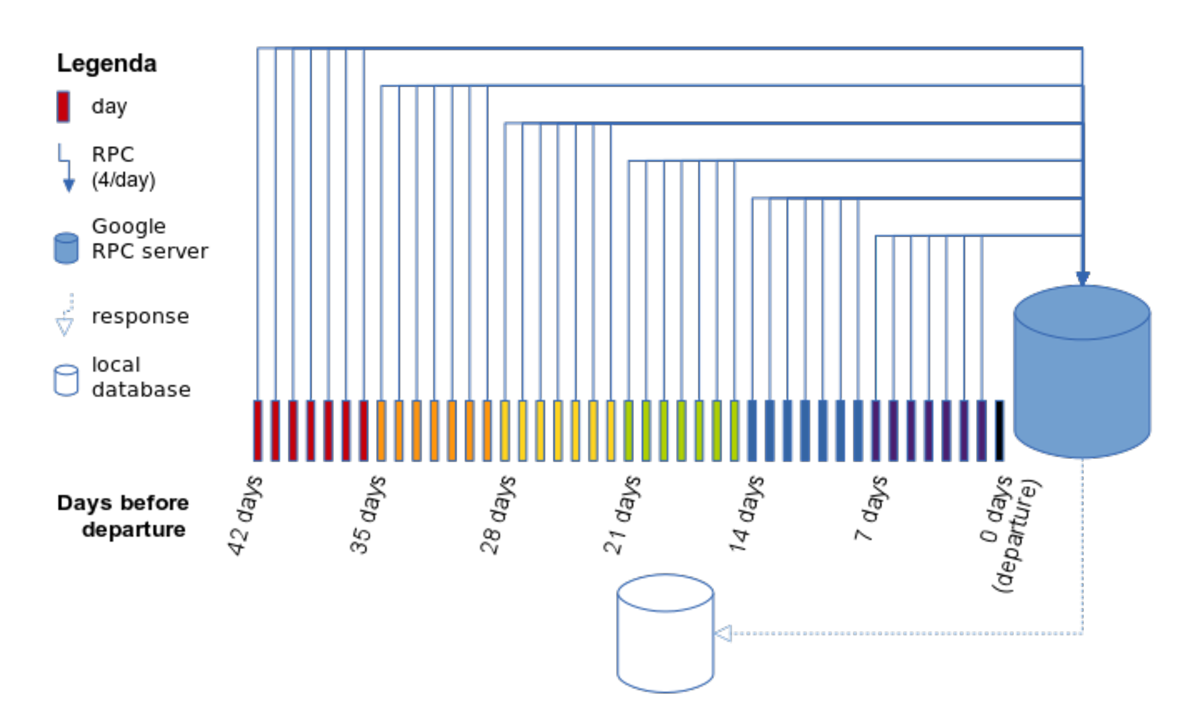
\includegraphics[width=0.8\textwidth]{figures/DataRetrievalProcess}
\caption{Data retrieval process}
\label{fig:DataRetrievalProcess}
\end{figure*}

Data will be collected on the previously mentioned routes departing during the period from Monday the $19^{th}$ of August up until Sunday the $29^{th}$ of September. Price data on all these flights will start 6~weeks prior to departure, up until the day before take-off. The data retrieval can best be illustrated with the help of \autoref{fig:DataRetrievalProcess}. Each day (represented by a rectangular box) an automated program will send a \emph{Remote Procedure Call} (blue arrow) to the \emph{RPC-server} of Google Flights (blue cylinder). This request asks the server to send data on a flight that meets certain specifications. For example, the first call the program makes on July the $8^{th}$ (6~weeks prior to start of collection of specific route) is ``\emph{return data on all flights from ATL to MCO departing on August $19^{th}$ and returning on August $26^{th}$ (7 days after departure)}''. The call is send to the server as a JSON-formatted request (See \autoref{app:SampleJSONRPC} for an example). In return, Google's server will send data on all the flights that meet those requirements (blue dashed arrow) and the automated program will store the received information in a local database (white cylinder). Because Google Flights does not always send back the same flights, the same RPC is send every 6~hours (at 00:00, 06:00, 12:00 and 18:00) \footnote{Each blue arrow thus represents 4 requests on that single day}. The next day the same process is repeated by sending the exact same query to the RPC-server again. This procedure is repeated each day up until the day before departure.

The illustrated process only describes one route (i.e., \emph{ATL} to \emph{MCO}) on one specific date (i.e., departure on \emph{August $19^{th}$}). The automated program however takes into account every route described in \autoref{app:selectedroutes}, and all dates in the period from August $19^{th}$ till September $29^{th}$. The total number of requests made to Google's RPC-server is thereby 22,176 calls \footnote{4 times per day for 7~days per week for 6~weeks for each 22~flights for a period of 6~weeks}.

After retrieval of the flight information, the data is parsed and stored in the \href{http://www.hdfgroup.org/HDF5/}{HDF5-format}. This data format is often used in big data analysis, and enables quick reading of big sets of data to memory. Following the loading into RAM, the data will be converted to a \href{http://pandas.pydata.org/}{Pandas} object after which analysis can be done.

Distinction between flights is made by hashing flight's  properties\footnote{The \emph{call sign} of each segment and \emph{ticketing code} of the flight}. Prices of the flight will be stored in the HDF5-file using the hash as the identification key. This enables easy extraction of price fluctuations within exact same flights relative to time.

\subsection{Option valuation models}
\label{subsec:OptionValuationModels}

% Mun 2006 [jain]: daily return calculation

In this phase the models for option valuation will be built. Currently airliners that offer options on their flights, offer these at a fixed price. This price only differentiates on maturity date, and is equal for all flights and time of purchase. For instance, customers are presented the same price when purchasing the option 1~day or 4~weeks before departure. See \autoref{tbl:PriceOfAirfareLockIn} for examples of current prices at which aviation companies offer fare lock-in products.

\begin{table}[ht]
	\centering
	\begin{tabular}{l  c  c  c  c}
	\hline \hline
	Airline         & 2~days & 3~days  & 7~days  & 14~days \\ \hline
	United Airways  &        & \$\,5.99 & \$\,8.99 & 	       \\
	Air France-KLM  &        &         &         & \$\,20   \\
	Estonian Air    & \$\,15   &         &         &         \\
	\hline
	\end{tabular}
	\caption{Price of airfare lock-in}
	\label{tbl:PriceOfAirfareLockIn}
\end{table}

In this research I will compare three different types of option pricing methods, name\-ly \begin{inparaenum}[\itshape (i)\upshape]
\item an optimal model based upon foreknowledge,
\item a theory-based approach based upon the Black--Scholes model, and
\item a numerical approximation approach based upon the Monte~Carlo method.
\end{inparaenum} The first model is is the theoretical optimal method, while the latter are practically feasible.

\subsubsection{Theoretically optimal: foreknowledge}
The first option valuation model built in this research is based upon the assumption that the option seller knows the exact price of the underlying flight in the future. While this is infeasible in practice, this theoretical model will provide the answer to the first~research question. By using this technique one can conclude whether the external company is able to provide options at a price which the passenger accepts. If it is viable to offer such option in this theoretical setting, more realistic models can be built to see whether it is also feasible in the practical world. Furthermore, this optimal method will be used as baseline to compare the other two models. 

\subsubsection{Theory-based: Black--Scholes model}
The Black--Scholes model will be the first practical implementations of a option valuation technique in this research. The model is used to determine the European option price based upon the volatility of the underlying asset. \citeA{jain11} demonstrated in their paper that this model can also be used to determine optimal option prices based on the volatility of airfares. In this paper, I calculate the volatility of the airfares by using the first 4~weeks of the census. With this variable, the optimal option price according to the Black--Scholes method can be calculated, and the outcome can be tested in the simulation model. The adapted equation used for this flight specific scenario is derived from \citeA[p.~13]{jain11}:
\begin{align*}
p_O &= p_I \times N(d_1) - p_S \times e^{-rT}N(d_2) \\
d_1 &= \frac{\ln(p_I/E) + (r + \sigma^2/2)T}{\sigma \sqrt{T}} \\
d_2 &= d_1 - \sigma \sqrt{T}
\end{align*}
See \cref{app:AdaptedBlackScholesFormula} for a full description of the equation.

\subsubsection{Numerical approximation: Monte Carlo}
The next practical implementation of an option valuation technique is the Monte~Carlo method. This model is more flexible and can be used when the underlying returns do not follow a log-normal distribution. Furthermore, as \citeA{walker1998method} states, options on flights are quite different from options found in the financial market. The main differences are \emph{non-interchangeability} and \emph{capacity restrictions}. A Monte~Carlo can be configured in such a way that it also takes into account such distinctions.

\citeA{richardson2009numerical} gives an example implementation of the Monte~Carlo method to set the prices of options. Instead of volatility and random returns, I will implement this model based upon the expected returns seen in the training~set of the data. The outcomes will be tested using the designated set of the data, and relatively compared with the optimal model.


\subsection{Simulation and sensitivity analysis}
\label{subsec:SimulationAndSensitivityAnalysis}
In the third phase the three pricing models described in \typenameref{subsec:OptionValuationModels} will be evaluated using simulation.

This simulation model generates passengers that want to buy tickets of a certain flight as a function of time (6~weeks till one day before departure). 

To make sure the models are not overfitted on the train data, the simulation will be run on the separate set of test data.

\subsubsection{Sensitivity Analysis}
During the simulation a sensitivity analysis will be performed as well. In this analysis the three~parameters of a passenger --- \begin{inparaenum}[\itshape (i)\upshape]
\item risk-utility,
\item forecasting technique, and
\item likelihood of travelling.
\end{inparaenum} --- will be altered to see what the effect of these properties is on the price setting model.

\chapter{Model development}
\label{chap:ModelDevelopment}
This chapter will discuss the simulation model used for the evaluation of the option pricing techniques. \todo{descr}

\section{Simulation model}
\label{sec:SimulationModel}
In this thesis, a series of simulations will be run to determine the performance of different option valuation models. These pricing models range from theoretical optimal --- the seller with perfect foresight --- up till the practically implementable --- based upon historical prices and Monte~Carlo simulation.

The first simulation run will determine the maximum possible profits an option seller could realize. The results will be acquired by assuming an option writer that has perfect information on price movements and customer characteristics, and thus acts accordingly. Though these assumptions are unrealistic in a real word setting, the observations of this run can be used as the benchmark to compare the performance of other option models to.

The runs after the optimal case will drop some of the assumptions made about the seller with perfect foreknowledge, and determine the influences of those assumptions on the results. The final case will be a practically implementable option valuation model based upon historical prices.

To determine the outcomes associated with each of the models, each simulation will run through a number of steps. This process is illustrated in \autoref{fig:simulationProcess}. The processes above the line are the ones associated with the buyer, the demand side. The ones below are connected to the airfare~lock-in product seller, the supply model.

\insertfigure{simulationProcess}{Illustration of simulation process}

The process shown in the figure can be described in more detail using the seven~consecutive steps:

\begin{description}
\item[Arrival of passenger] In the first stage of the simulation, the model will generate the arrival of passengers. A passenger is interested in buying an airfare~lock-in product on a specific flight. The simulation does not calculate the customers willingness to pay for the ticket price, but assumes that they all in principle want to buy the ticket at the current fare. Therefore, the model only determines whether the customer wants to buy the option on the flight.

In this research, I will generate passengers according to a homogeneous Poisson distribution with an average arrival rate of 1 customer per option per day before departure ($\sim \mbox{Pois}(\lambda=1)$). The use of a (non-)homogeneous Poisson distribution is common in literature on simulating arrivals for flights (e.g., \citeA{2007simulation}, \citeA{bertsimas2005simulation}, \ldots).

Because data have been collected on flights up till 42~days before departure, each ticket will receive this same number of passengers with option requests on average. However, because when selling options with a specific number of days to maturity $m$ it is not possible to buy options fewer that $m$ days to departure, these customers get excluded from the model. As an example, the test dataset containing airfares of tickets from LHR to JFK includes 7,690 unique flights after cleansing. When simulating this model for options with a maturity of 3 days an expected total of $(42 - 3) \times 7,690 = 299,910$ passengers will be generated. Due to the probabilistic outcomes of the Poisson distribution, the exact number of arrivals number might vary.

\item[Calculate the passenger's WTP] The next step of the simulation will engage itself in the calculation of the customer's Willingness To Pay. This amount is determined by computing the minimum of the expected utility of buying the flight immediately, or postponing the decision to fly $m$~days later.

The exact level of a customer's WTP is dependant on three other variables. These variables are
\begin{compactitem}
    \item the customer's forecasting method of the expected increase in airfare,
    \item the accuracy of the customer's forecasts, and
    \item the likelihood of travelling.
\end{compactitem}
The implementation of these concepts is explained in detail in \todo{ref}.

Now that the customer knows his level of WTP, he requests the seller for the price of the option.

\item[Calculate the option seller's WTA] The third step is responsible for the computing the option seller's minimum \emph{Willingness To Accept}. A writer's WTA is the minimum level at which the seller wants to offer options that insure against price risks. When he would offer the airfare~lock-in products at this value, the seller would not expect any returns on the sale. The WTA of the external party is thus calculated using the writer's predictions of how the airfare is expected to change.

The simulation model in this thesis uses many different configurations for the option sellers. In the benchmark case, a lock-in product seller with perfect information is considered. His WTA for each option is the same as the observed level of increase of the underlying fares. The different methods for computing the WTA for every particular configuration of the writer will be described in detail in \todo{ref}.

\item[Calculate the price of the option] Step number four will calculate the price at which the option will be offered to the passenger. This simulation will calculate this value by either setting it to the customer's exact degree of WTP, or by applying a margin on top of the WTA calculated in previous step. To ensure that the seller does not offer options for a negative revenue --- which could be the case when he expects a decrease in airfare --- also a minimum price is set. All calculated option prices that fall below this set minimum price will be raised to this level. After computing the option price, the customer then gets offered the option at this fare.

\item[Acceptance of the offer] The next step will determine whether the customer will accept the airfare~lock-in product offer. This is done by comparing the customer's WTP and the offered option price. When the Willingness To Pay of the customer for a certain flight is higher than the option price calculated in prior process, a customer will accept the offer (i.e., $\text{WTP} \ge p_O$).

\item[Exercising the option] The second-last step in the simulation process will determine whether the customer will actually exercise his option at the date of maturity. To do so, the model will first `wait' $m$~days, and check the observed ticket price. A customer will only exercise its right when this observed airfare is higher than the strike price of the option, $p_S$. Furthermore, the passenger will only use the option when he has decided to fly. When both of these rules apply to a certain customer, he will thus make use of his lock-in product, and let the seller buy the flight ticket for him.

\todo{decision tree}

\item[Calculate generated outcomes] The final step in the model will calculate the outcomes of each sold option. When the customer does not exercise his option on the date of maturity, the seller will gain the full price at which he has sold the option in profits. When the passenger actually does exercise his right, the profits or losses gained from selling the option can be defined as:
$$ y = p_O - (p_S - p_m) $$
\end{description}

Using the method described above, the simulation will be used to compare the performance of the proposed option valuation models. The same procedure will also be used to test the influence of a particular configuration of parameters within a single option valuation model.




\subsection{Structure of the model}
In this research, two different submodels are being considered. The first one --- the \emph{demand submodel} --- is concerned with the option valuation on the customer's side. This submodel calculates the willingness to pay for an option from the perspective of the passenger determining whether to buy the product. The \emph{supply submodel}, on the other hand, computes the willingness to accept from the seller's view.

\subsubsection{Demand submodel}
The demand submodel concerns itself with the calculation of the willingness to pay on the passenger's side of the model. To compute his willingness to pay, the customer uses the following equation:

$$ \mbox{WTP}_c = E[V_c] \times P^f $$

Where $P^f$ is the customer's likelihood of travelling and $E[V_c]$ is the customer's expectation of the standard option price. In this thesis, \emph{standard option price} refers to the value of an option that a customer would be willing to pay when his $P^f$ is equal to 1.

The customer's expectation of the option price is calculated using a specific prediction method. In this research, the customer will base these forecasts on his \emph{rational expectations} (RE) of ticket price movements. This type of prediction method was first introduced by \citeA{muth1961rational}, and later generalized to also include more cases by \citeA{arrow1962economic}. The expectations generated from the RE-model assume that the entity makes rational predictions based upon all the information he has, plus a random \emph{error term}. In the strong case, the RE-model assumes the entity's predicted values are the actual observed prices plus a random fluctuation. The weak case, however, assumes the customer will base his forecasts only on available (historical) information, $I_0$. Because this information might differ from the actual observed values, this method is expected to be less accurate.

For the passenger, I will consider two types of rational expectations:

\paragraph{Strong-form rational expectation (used in benchmark)}
In the strong-form case, the customer will base his expectations based upon the actual price changes as seen in the future:

$$ E[F_m] = F_m \times \epsilon$$

The random error in the equation will be drawn from a normal distribution with mean 0 and a specified standard deviation:
$$ \epsilon \sim \mathcal{N} (0, \sigma^2) $$

A higher standard deviation will thus lower the accuracy of the passenger's expectations.

The resulting prediction $E[F_m]$ will be a point estimate which represents the expected future airfare according to the customer. To compute his standard option price, the passenger will subtract the current ticket price from the acquired point estimate:

$$ E[V_c] = E[F_m] - F_0$$


\paragraph{Weak-form rational expectation}
When applying the weak-form case of rational expectation, the customer will base his expectations upon the historically observed changes:

$$ E[F_m] = (E[F_m] | I_0) \times \epsilon $$

Where $I_0$ represents the historical distribution of price changes of the current route.

Like in the strong-form RE, the random error term in the above equation will be drawn from a normal distribution with mean zero and a standard deviation. A higher standard deviation also results in lower accuracy of the passenger's predictions.

From the historical distribution, this form of rational expectation will construct an expected distribution of price changes of the current airfare. Next, the expected distribution of fluctuations is used to calculate the anticipated ticket price at the option's date of maturity:

$$ E[F_m] | I_0 = \sum |F_m \times P[F_m]| $$

The customer's standard option price is then computed by subtracting the current airfare from the expected future fee:
$$ E[V_c] = E[F_m] - F_0 $$

For the benchmark, the simulation assumes that the customer will base his expectations using the \emph{weak-form rational expectation} method. After the computation of the passenger's standard option price, his willingness to pay has to be determined using his probability of flying.

\paragraph{Passenger's likelihood of travelling}
The passenger's likelihood of travelling gives the probability that he will decide to fly when his option matures. Each passenger's $P^f$ is being simulated by drawing a random value from a uniform distribution between zero and one:

$$ P^f \sim \mbox{Unif}(0, 1)$$

Every customer thus has his own random value of $P^f$. The model assumes the customer knows the \emph{exact} level of this probability, and acts accordingly. As shown in \todo{ref}, this probability of flying influences the passenger's willingness to pay of an option linearly; a low $P^f$ results in a low likelihood of actually having to use the option, while a high probability leads to a higher likelihood of having to exercise the product at maturity. The customer's willingness to pay for an option thus is the standard option price times this probability.

As stated in previous section, the customer will accept the option if his willingness to pay is greater than or equal to the offer he receives from the seller:

$$ \mbox{WTP}_c \ge V_s $$

The methodology for how the seller sets the price of the option, $V_s$, is described in detail in \todo{ref}.

As can be reduced from the equation for calculating the WTP, this simulation model assumes \emph{risk neutral} customers. However, research has shown this is unlikely the case as real option buyers tend to be risk averse (see for example \cite{miller2004empirical}). As risk aversion leads to a higher willingness to pay, the results yielded from this simulation will probably be lower. The inclusion of risk neutrality is a conservative assumption, but allows for a more simplistic model. Also, when future research decides to implement risk averse buyers in the model, the results will mainly be better; if the concept yields positive results in a risk neutral setting, it will most likely do so as well in a risk averse scene.

\paragraph{Exercise of the option}
On the date of maturity, a Bernoulli trial will be run to determine whether the customer will actually fly. When the outcome of the trial is $0$, the customer has decided to \emph{not} travel and thus make no use of the option. When the outcome of the trial is $1$, the customer has decided that he will make use of the flight.

\begin{equation}
\sim \mbox{Bernoulli}(P^f)\begin{cases}
     \mbox{fly}, & \mbox{if } 1 \\
    \mbox{don't fly}, & \mbox{if } 0 \end{cases}
\end{equation}

Due to this property, the passenger will thus always receive information on the date of maturity on whether he will fly.

After the Bernoulli trial, the customer will have to decide whether he will exercise his option. This is the case when the following applies:
\begin{compactitem}
    \item the ticket price on the option's date of maturity is lower than the strike price, ($p_S < F_m$) and
    \item the customer \emph{does} want to make use of the flight.
\end{compactitem}

He will thus \emph{not} exercise his option when:
\begin{compactitem}
    \item the ticket fee on the option's date of maturity is higher than the strike price ($p_S > F_m$), or
    \item the customer does \emph{not} want to make use of the flight.
\end{compactitem}

\todo{tree}


\subsubsection{Supply submodel}
Like the demand submodel, the supply submodel concerns itself with determining acceptable option prices. However, this model computes the prices from the perspective of the seller. This thus means that instead of calculating a willingness to \emph{pay}, the supply submodel tries to determine the best willingness to \emph{accept}. It does so by using the following equation:

$$ WTA_s = \max(V_{min} \times F_0, E[V_s] \times M) $$

Where $V_{min}$ is the minimum option price in percentages of current airfare, $F_0$ is the current airfare, $E[V_s]$ is the expected standard options price according to the seller, and $M$ is the margin.

The first part of the equations ensures that there is always set an option price higher than zero. This is to prevent situations from happening where the seller thinks the airfare will go down at the date of maturity, and asks a negative option price (i.e., he would offer the customer money for buying the customer). This is of course an undesirable effect which is averted by setting a minimum price relative to the current airfare.

To calculate the expected option price, the seller can also make use of three different prediction methods.

\paragraph{Perfect foresight (used in benchmark)}
In the simulation where the seller has perfect foresight, it can 100\,\% accurately predict price changes of a flight. Though this is not a realistic assumption for a real-world setting, it gives valuable insights and will be used as an `optimal' benchmark to compare the other simulation models with.

\paragraph{Strong-form rational expectation}
The strong-form rational expectation model uses the same underlying technique as the strong-form case of the customer's prediction method. This model is being used as a `black box' to represent a relatively accurate prediction system implemented by a company. While there is too limited time and resources in this research to actually develop such a forecasting model, research has shown that accurate models can be developed (\todo{ref}). In this simulation the model thus assumes such a prediction model has been developed and implemented.

\paragraph{Monte Carlo}
The last forecasting method of the seller to determine its preferred option prices makes use of the Monte Carlo method. This is a practical forecasting model that can be easily implemented in a realistic setting. The model only uses historically available information obtained from the training set, so any predictions made in this model could also have been made when the test set was not available yet. When this model will yield positive results, it shows that even with a simplistic model the airfare~lock-in product business model could be viable.



\subsection{Parameters and assumptions of the simulation model}
Next to previously defined submodels, a number of entity characteristics and parameters have been defined. The next section will describe these variables, and define the configuration for the baseline which is being used for the initial simulation. The simulation models in later sections (e.g., \todo{ref}) will loosen the specified parameters to see its effects on the performance of the parameters itself.

In this research, a parameter is defined as a variable of the underlying object which can be altered to represent different values. The sensitivity analysis will thus adjust some of these parameters, and determine their influence. For example, the number of days till maturity of an airfare~lock-in product can hold the values 3, 7, 14, or 21~days for different simulation runs.


\subsubsection{Characteristics of the flight ticket}
\label{sub:CharacteristicsOfTheFlightTicket}
The first entity represents the ticket for a flight. A ticket gives its holder the right to take a seat on a particular underlying flight. In this thesis, a specific set of flights is being used:

\begin{compactitem}
\item each flight is for a specific route between outbound and inbound airport;
\item only single-legged (direct) flights are being considered;
\item only round trip flights are being considered;
\item each flight has a specific departure date;
\item the return date of the flight is always 1~week after the departure date.
\end{compactitem}

\vspace{1em}

Each ticket also has a certain price. This price can differ depending on the lookup~time of the ticket. In this research, airfare changes have been monitored up to six~weeks (i.e., 42~days) prior to departure. A certain price of a ticket can thus be defined in the number of \emph{days before departure}, or \emph{dbd}.

Lastly, the simulation model used in this research makes the assumption that the underlying tickets are non-transferable and non-refundable. The customer is therefore \emph{not} able to buy a ticket and get a refund at a later time, or transfer it to another person or departure date. This is essential for the concept of options to work, as else the passenger will likely always buy the ticket immediately at arrival and request a refund when he is unable to fly.

During this thesis, a data set of airfares on flight tickets for 22~different routes was collected during a period of 12~weeks. The empirical data acquired in this stage are being used in the simulation model. The complete analysis on these airfares is given in \autoref{chap:DataAnalysis}.


\subsubsection{Characteristics of the airfare~lock-in product}
The next entity which is being considered in this simulation model is the airfare~lock-in product. This product gives its holder the right --- but not the obligation --- to buy the underlying flight. There are two parameters associated with the entity. Unlike for financial options, the model assumes that the options on flights are non-transferable. When a customer thus decides he won't be exercising the ticket, he \emph{cannot} sell the airfare~lock-in product to another customer.

\parameter{the option's number of days till maturity \hfill ($m = 3$)}
The first parameter of the airfare~lock-in products is its number of days till maturity. This value denotes the number of days of extra \emph{decision time} a customer gains when he buys the option. At the date of maturity, the customer has to make the decision to actually buy the ticket, or to not exercise the option at all. A passenger will choose for the first alternative when he has decided to actually fly, and the current airfare is higher than the agreed upon \emph{strike price}. During this number of days $m$, the customer is thus \emph{insured} against price fluctuations and will therefore not risk high fare increases.

In the baseline model of the simulation, a maturity of 3~days is being considered. When a passenger thus purchases the option, he will decide whether to exercise the option 3~days after the acquisition of the lock-in product.

\parameter{the option's strike price \hfill ($p_S = p_I$)}
The second parameter associated with the entity is the strike price of the airfare~lock-in product. This price, denoted by $p_S$, is the cost at which the passenger is able to buy the underlying flight ticket when he exercises the option.

This research will consider a strike price of the airfare~lock-in product that is equal to the initial airfare of the underlying flight at purchase of the option.
$$p_S = p_I$$

For example, when the current ticket price $p_I$ is equal to \$\,100 and the customer decides to buy the option, he has the opportunity to buy the ticket for \$\,100 at the date of maturity.

Next to these configurable parameters, an airfare~lock-in product also has a certain price at which the option is offered to the customer. The theoretical level of this option price is described in \typenameref{subsec:PassengersWTP}. In this research, however, a number of different option valuation techniques are being considered. These pricing models are characterized by different configurations of the parameters of this simulation model, and will be described in detail in \autoref{chap:Results}. \todo{edit}


\subsubsection{General characteristics of the simulation model}
Next to the parameters and assumptions specific to the four entities described previously, the simulation model itself also has some characteristics defined.

\parameter{arrival rate of passengers \hfill $\sim Poisson(1)$}
As seen in the process description of the simulation (see at the beginning of this chapter), the model will generate passengers to determine the performance of the model. A passenger will arrive following a Poisson distribution with $\lambda = 1$. This thus implies that, on average, a single customer arrives for each day prior to departure for every flight.

\parameter{number of trials \hfill (N=20)}
Because pseudo random generation of numbers and probabilities are used in this model, there is a possibility of generating outliers in only a single run. To prevent such scenarios from happening, every simulation is run a number of times. The acquired data from these multiple trials is then averaged to get the converged mean.

A tests showed that the results converged to a mean at around 10~simulation runs. The rest of the simulations will therefore use a minimum of 20~trials before evaluating the results.

Lastly, to be able to compare the models even beter amongs themselves, the same random seed is set prior to running each simulation. This ensures the routes will receive the same `randomly' generated input for passenger arrival, error, et cetera.
\chapter{Data analysis}
\label{chap:DataAnalysis}
This chapter will engage in the analysis of the acquired flight data from Google Flights. The first part will describe the obtained data. Furthermore, it will describe the cleaning process of the observations, as well as the oulier analysis. The second part will focus on the descriptive analysis of the datasets.

\section{Data description and cleansing}
Flight ticket prices were collected for a period of 42~days ranging from the $9^{th}$ of July till the $29^{th}$ of September. During this data collection phase, airfares on the 22~routes described in \autoref{app:SelectedRoutes} were gathered on flights departing from the $20^{th}$ of August till the $30^{th}$ of September. In these 12~weeks, 158,410~files were requested from Google~Flights' RPC-servers, which resulted in a set of almost 18~gigabytes of JSON~data. Fifteen of these requests failed at the first try, and had to be downloaded again one quarter of an hour later. Of these retries, the automated script also failed to download 2~files at the second request. These failures were the request made on the $20^{th}$ of September at 00:00 GMT+2 for flights departing from JFK to LHR on the $25^{th}$ of September and the request made on the $26^{th}$ of July at 00:00 GMT+2 for flights departing from LHR to LAX on the $1^{st}$ of July. Due to the methodology applied by this research, in which 4~daily time windows are aggregated into a single value, these 2~failures did not create any gaps of missing values in the final data matrix.

After retrieval of the data all the JSON-files were parsed for airfares of flights. As stated in \autoref{sub:CharacteristicsOfTheFlightTicket}, this research only includes single-legged round~trip flights between the defined 22~routes between outbound and inbound airport. The parsing of the files resulted in a matrix with rows containing a flight's fare history in 6~hour time windows. These windows were then converted into daily observed airfares. The conversion into daily values resulted in a database containing 462,662 unique flights which included 12,865,953 airfare observations. Due to Google Flights' nature of returning a limited set of airfares for each request, some flights did contain gaps of missing values within their data. In alignment with the study by \citeA{groves2013agent}, this paper therefore excludes flights for which less than $\frac{2}{3}$ of the possible airfare observations are available. So, because there are a total of 42~observations days prior to each flight, tickets that do have fewer points than $42 \times \frac{2}{3} = 28$ available will be excluded from the analysis. Next, because airlines are known to open and close specific price-buckets \cite{mcgill1999revenue}, some gaps were still present in the dataset. These gaps were filled with the data available from observations made in the future. For example, when a particular flight misses a price observation at 35~days before departure, but it does contain the airfare for 34 and 36~days prior to departure, the 35~days' window would be filled with the same value as the 34~days before departure. In reality this would mean that when a customer's option expires, but the ticket is not available on the date of maturity (i.e., no price observation). The customer thus would have to wait till the airline resumes the sale of that flight. He would therefore get the ticket at the price in the future.

Missing data at for the last (few) days prior to departure are considered to be the sell-out of a flight. Because Google Flights' also offers Business and First class tickets, this implies that all the seats are completely sold out, and there is no possibility of still buying the ticket. This means that when a customer's option expires on such a ticket and he wishes to exercise it, an alternative flight has to be offered. To prevent such situations from happening, these missing data on sold-out flights is filled with a penalty similar to the technique used by \citeA{etzioni03}. By introducing such a penalty, the option valuation model is triggered into trying not to offer options when the probability of sell-out is high. Instead of the \$300,000 proposed by the authors, I have chosen to set the penalty at 3 times the average airfare at 1~day before departure. This is more realistic in a sense that the customer could be offered an alternative flight that leaves on the same day plus some extra form of monetary compensation. Furthermore this lower fill-value prevents penalties from biasing the airfares closer to departure.

An illustration of this data filling process is given in \autoref{fig:dataFillingOfMissingValues}. Airfares are given as integers representing the price in cents. As can be seen in the figure, the n/a-gaps are filled with the nearest available future price closer to departure. Furthermore, the missing value for the flight with id~\#3 at 1~day before departure is seen as a sold-out ticket. This value is filled with $3 \times \bar{c_1}$, where $\bar{c_1}$ represents the average of the airfares observed at a single day before departure.

\begin{figure}
$$
\kbordermatrix{
           & 1\,\scriptstyle{dbd} & 2\,\scriptstyle{dbd} & 3\,\scriptstyle{dbd}  & \cdots \\
    \#1    & 10000                & 12000                & 12000                 & \cdots \\
    \#2    & 20000                & \mathrm{n/a}         & 22000                 & \cdots \\
    \#3    & \mathrm{n/a}         & 32000                & \mathrm{n/a}          & \cdots \\
    \vdots & \vdots               & \vdots               & \vdots                & \ddots
}
\Rightarrow
\kbordermatrix{
           & 1\,\scriptstyle{dbd} & 2\,\scriptstyle{dbd} & 3\,\scriptstyle{dbd}  & \cdots \\
    \#1    & 10000                & 12000                & 12000                 & \cdots \\
    \#2    & 20000                & 20000                & 22000                 & \cdots \\
    \#3    & 3 \cdot \bar{c_1}    & 32000                & 32000                 & \cdots \\
    \vdots & \vdots               & \vdots               & \vdots                & \ddots
}
$$
\caption{Data filling of missing values (i.e., n/a)}
\label{fig:dataFillingOfMissingValues}
\end{figure}

The empirical dataset shows that in total 15,643 flights are not offered (i.e., sold out) at 1~day before departure. These tickets take into account 5.6 percent of the all the flights available. Real-world data on the number of sold out flights is very hard to acquire, because this value could give sensitive information on the performance of an airline. However, this number of sold outs seems to be on the low side. A possible explanation for this might be that this research only requests airfares up till 1~day before departure. So, likely a higher number of sold outs will be observed when one also requests the fares on the day of departure. Furthermore, due to the time window averaging of the 4~daily fare observations, the daily value actually includes all ticket prices acquired 24~till 48~hours before departure.

After cleaning the dataset, it was split into two separate parts. The database used in this research contains airfare observations of flights departing in the period $20^{th}$ of August till the $30^{th}$ of September. As explained in \autoref{chap:Methodology}, the first 4~weeks of these departing flights --- $20^{th}$ of August till the $16^{th}$ of September --- will be used as the training set for the research. The latter 2~weeks --- from the $17^{th}$ of September till the $30^{th}$ of September --- will be used for testing the proposed option valuation models. This split resulted in a training set containing 321,545 flights, and a test set which includes 141,117 flights. An example extract of the final test data matrix used for the flights from AMS to JFK can be found in \autoref{fig:extractFromAMStoJFK}. In this extract, the flight with id~\#4 was sold-out 1~day before departure, and that field was thus filled with $3 \times$ the average ticket price at 1~day before departure.

\begin{figure}
$$
\kbordermatrix{
           & 1\,dbd & 2\,dbd & 3\,dbd & 4\,dbd & 5\,dbd & \ldots & 42\,dbd \\
    \#1    & 57469  & 68619  & 122469 & 222469 & 109644 & \ldots & 65853   \\
    \#2    & 87119  & 87369  & 93019  & 84469  & 79469  & \ldots & 65853   \\
    \#3    & 87494  & 86694  & 94744  & 74569  & 70244  & \ldots & 65853   \\
    \#4    & 410951 & 134430 & 242480 & 108934 & 126369 & \ldots & 123357  \\
    \vdots & \vdots & \vdots & \vdots & \vdots & \vdots & \ddots & \vdots  \\
    \#252  & 68984  & 69094  & 64669  & 73219  & 70244  & \ldots & 65857
}
$$
\caption{Sample extract from test data matrix AMS to JFK}
\label{fig:extractFromAMStoJFK}
\end{figure}



\subsection{Outlier analysis}
\label{subsec:outlierAnalysis}
After cleansing the dataset, the outlier analysis was performed. First, extreme and invalid prices were identified and removed from the dataset. Google Flights sometimes yielded with an impossible airfare for a flight, and it is more likely that such values were not prices, but rather codes for the website. For example, when Google Flights does currently not have recent price information on a flight, the ticket price was set at 3. This of course is an impossible price for a flight, even more so considering the prices returned are in cents. To exclude these codes from the dataset, all airfares lower than 1,000~cents were removed from the dataset (i.e., $p_i < 1000$).

For the next step of the outlier analysis, box plots of the observed ticket prices were generated. These plots are displayed in \autoref{fig:BoxplotsWithOutlierAnalysis}. The whiskers for these plots have been set to 1.5~times the interquartile range.

A quick analysis of these figures shows that there are many theoretical outliers available for each flight. In this research, however, I have chosen not to exclude these from the actual dataset. The reason for this is that these airfares have been empirically observed, and could therefore appear in a real world setting. These airfares could arise when the seats in the economy~class for that flight were sold out, and the cheapest available option was an upgrade to first or business~class. When these values would be removed from the dataset, a too optimistic view could arise. In such a view the simulated risk would be undervalued and profits would be overestimated. This would lead to a misfit between this research and the real world application, and the results would yield worthless.

Furthermore, as will be demonstrated in \autoref{subsec:DescriptiveAnalysisOfFareChanges}, the strong tendency of the data towards `no price change' could have lead to a underestimated standard deviation. Therefore, the box~plots might label some observations as outliers, while this is actually not the case.

Because of these reasons, I have decided to not exclude these observed outliers from the dataset.


\begin{figure*}
\centering
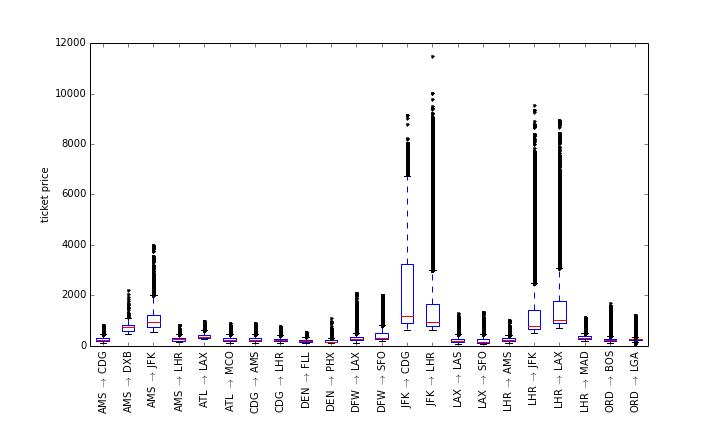
\includegraphics[width=.8\textwidth]{figures/outlierAnalysis}
\caption{Box plots with outlier analysis}
\label{fig:BoxplotsWithOutlierAnalysis}
\end{figure*}


\section{Exploratory data analysis}
In this section the exploratory data analysis is performed on the dataset after cleansing. First, a descriptive analysis is performed on the number of flights, observations and sold outs of both datasets. Next an analysis is performed on the ticket prices and daily price fluctuations. This analysis also includes a test of normality to see whether the distribution follows a normal distribution. Lastly, a comparison between the training and the test dataset is made to see whether they differ significantly.

Throughout this research, a distinction is made between two databases, namely: the training and the test dataset. The \emph{training} dataset will be used as historical airfare information on which the customer bases its forecasts. Furthermore, the training dataset is also used by the seller in the Black--Scholes and Monte~Carlo models to compute his Willingness To Accept. The \emph{test} set is used to evaluate the option pricing models.

\subsection{Descriptive analysis of flights}
First, the descriptive analysis on the flights is performed. The results of this analysis on all the flights available in the total dataset, as well as the distinction between test and training, can be found in \autoref{tbl:DescriptiveAnalysisTotalDataset}. The \emph{Flights -- total} row displays the total number of unique flights available in the specified dataset. \emph{Flights -- valid} shows the count of flights that exceed a certain threshold of daily observations made for that route. As stated in \autoref{chap:Methodology}, only flights with more than 28~observations\footnote{Two-thirds of the total 42~possible observations} are included in the analysis. The \emph{Fares -- total} line gives the total number of airfare observations made in the dataset containing only the valid flights. The last two rows specify the number and percentage of sold outs in the data.

As one can deduce from this analysis, the training set is significantly larger than the test data. This is due to the split in empirical data. The first 4~weeks of the set are assigned to the training dataset, while only the latter 2~were selected to be the census for the test set. In a real world application of option valuation models this is likely to be also the case, as there is much more historical data available to the option seller than there are flights on which he has to make forecasts for. The difference in counts in both datasets is not expected to be of influence on the results of the simulation model, as there are a vast amount of data available to both sets.

The costs due to sold outs, however, is expected to be higher due to the difference between both sets. The Black--Scholes and Monte~Carlo models both base their predictions upon the historical (i.e., training) dataset, and will therefore likely expect an equal amount of sold outs of flights in the test set. However, as can be seen from the data, the test dataset contains about 15~percent more sold outs than the training dataset.

\begin{table}
\centering
\footnotesize
\begin{tabular}{l l r r r}
    \toprule
    ~         &  ~          &  Total dataset  & Test dataset  &  Training dataset \\ 
    \midrule
    Flights   &  total      &  462,662    &  141,117    & 321,545 \\
    ~         &  valid      &  278,349    &  98,916     & 179,433 \\
    ~         &  valid (\%) &  60,2       &  70.1       & 55.8 \\
    Fares     &  total      &  11,280,278 &  4,064,937  & 7,215,341 \\
    Sold outs &  total      &  15,643     &  6,053      & 9,590 \\
    ~         &  total (\%) &  5.6        &  6.1        &  5.3 \\
    \bottomrule
\end{tabular}
\caption{Descriptive analysis total dataset}
\label{tbl:DescriptiveAnalysisTotalDataset}
\end{table}


A route-specific descriptive analysis of both datasets can be found in \autoref{tbl:DescriptiveAnalysisTestDataset} and \autoref{tbl:DescriptiveAnalysisTrainingDataset}.


\begin{table}
\centering
\footnotesize
\begin{tabular}{c c | c c c | c | c c}
\toprule
\multicolumn{2}{c|}{Airport}  & \multicolumn{3}{c|}{Flights} & Fares & \multicolumn{2}{c}{Sell outs} \\[.4ex]
from &  to  & total  & valid  & valid (\%)  &  total  &  total  &  total (\%) \\
\midrule
AMS  &  CDG  &   4,630  &   3,936  &   85.0  &  164,706  &    146  &   3.7 \\
~    &  DXB  &      14  &      14  &  100.0  &      588  &      0  &   0.0 \\
~    &  JFK  &     252  &     252  &  100.0  &   10,572  &      6  &   2.4 \\
~    &  LHR  &   2,834  &   2,558  &   90.3  &  106,611  &    108  &   4.2 \\[.5ex]
ATL  &  LAX  &   1,776  &   1,421  &   80.0  &   59,225  &      3  &   0.2 \\
~    &  MCO  &   4,727  &   3,757  &   79.5  &  156,488  &     24  &   0.6 \\[.5ex]
CDG  &  AMS  &   4,149  &   3,936  &   94.9  &  165,125  &     94  &   2.4 \\
~    &  LHR  &   1,264  &   1,250  &   98.9  &   52,437  &     14  &   1.1 \\[.5ex]
DEN  &  FLL  &      21  &      21  &  100.0  &      865  &      4  &  19.0 \\
~    &  PHX  &   1,541  &   1,453  &   94.3  &   60,847  &     50  &   3.4 \\[.5ex]
DFW  &  LAX  &  11,157  &   8,872  &   79.5  &  368,838  &    467  &   5.3 \\
~    &  SFO  &   5,272  &   4,503  &   85.4  &  182,895  &    578  &  12.8 \\[.5ex]
JFK  &  CDG  &   2,569  &   1,782  &   69.4  &   73,119  &    146  &   8.2 \\
~    &  LHR  &  10,824  &   7,918  &   73.2  &  331,646  &    182  &   2.3 \\[.5ex]
LAX  &  LAS  &   7,642  &   5,334  &   69.8  &  208,889  &    431  &   8.1 \\
~    &  SFO  &  32,367  &  16,161  &   49.9  &  653,809  &  1,317  &   8.1 \\[.5ex]
LHR  &  AMS  &   2,788  &   2,567  &   92.1  &  107,431  &     50  &   1.9 \\
~    &  JFK  &   9,981  &   7,690  &   77.0  &  322,109  &    159  &   2.1 \\
~    &  LAX  &   1,581  &     837  &   52.9  &   34,580  &     58  &   6.9 \\
~    &  MAD  &   4,758  &   4,732  &   99.5  &  198,705  &     26  &   0.5 \\[.5ex]
ORD  &  BOS  &   9,037  &   7,204  &   79.7  &  287,993  &  1,140  &  15.8 \\
.    &  LGA  &  21,933  &  12,718  &   58.0  &  517,459  &  1,050  &   8.3 \\
\bottomrule
\end{tabular}
\caption{Descriptive analysis of test dataset}
\label{tbl:DescriptiveAnalysisTestDataset}
\end{table}


\begin{table}
\centering
\footnotesize
\begin{tabular}{c c | c c c | c | c c}
\toprule
\multicolumn{2}{c|}{Airport}  & \multicolumn{3}{c|}{Flights} & Fares & \multicolumn{2}{c}{Sell outs} \\[.4ex]
from &  to  & total  & valid  & valid (\%)  &  total  &  total  &  total (\%) \\
\midrule
AMS  &  CDG  &   8,389  &   7,871  &  93.8  &  329,235  &    136  &   1.7 \\
~    &  DXB  &      35  &      28  &  80.0  &    1,176  &      0  &   0.0 \\
~    &  JFK  &     639  &     638  &  99.8  &   26,796  &      0  &   0.0 \\
~    &  LHR  &   5,380  &   4,891  &  90.9  &  204,906  &    110  &   2.2 \\[.5ex]
ATL  &  LAX  &   3,613  &   3,203  &  88.7  &  133,976  &      8  &   0.2 \\
~    &  MCO  &   8,554  &   7,602  &  88.9  &  317,860  &     39  &   0.5 \\[.5ex]
CDG  &  AMS  &   8,186  &   7,874  &  96.2  &  329,613  &    107  &   1.4 \\
~    &  LHR  &   2,577  &   2,529  &  98.1  &  106,218  &      0  &   0.0 \\[.5ex]
DEN  &  FLL  &      58  &      45  &  77.6  &    1,792  &      6  &  13.3 \\
~    &  PHX  &   2,433  &   2,426  &  99.7  &  101,656  &     89  &   3.7 \\[.5ex]
DFW  &  LAX  &  36,579  &  14,845  &  40.6  &  559,879  &    247  &   1.7 \\
~    &  SFO  &  16,117  &   7,436  &  46.1  &  279,339  &    313  &   4.2 \\[.5ex]
JFK  &  CDG  &   4,947  &   3,238  &  65.5  &  132,385  &    354  &  10.9 \\
~    &  LHR  &  23,440  &  14,825  &  63.2  &  610,280  &  1,489  &  10.0 \\[.5ex]
LAX  &  LAS  &  16,261  &   9,782  &  60.2  &  385,907  &    319  &   3.3 \\
~    &  SFO  &  68,886  &  24,929  &  36.2  &  988,534  &  1,928  &   7.7 \\[.5ex]
LHR  &  AMS  &   5,230  &   4,904  &  93.8  &  204,973  &    193  &   3.9 \\
~    &  JFK  &  22,540  &  14,711  &  65.3  &  606,489  &  1,039  &   7.1 \\
~    &  LAX  &   3,513  &   1,597  &  45.5  &   64,877  &    289  &  18.1 \\
~    &  MAD  &   9,464  &   9,438  &  99.7  &  395,966  &     67  &   0.7 \\[.5ex]
ORD  &  BOS  &  24,145  &  12,904  &  53.4  &  493,077  &  1,624  &  12.6 \\
~    &  LGA  &  50,559  &  23,717  &  46.9  &  940,407  &  1,233  &   5.2 \\
\bottomrule
\end{tabular}
\caption{Descriptive analysis of training dataset}
\label{tbl:DescriptiveAnalysisTrainingDataset}
\end{table}


The number of flights with a valid number of fare observations differs a lot amongst some routes. For example, the route AMS to DXB only has a single observation per data collection day, while a route like LAX to SFO contains almost 25,000~valid flights in the training set. This high difference has to do with the number of single-legged flights available on each route. AMS to DXB offers only a single option every day, which is operated by a single airliner (KLM). Hence, it only returns a single valid round~trip flight for each day. The route between LAX and SFO, however, offers around 50~direct flights operated and ticketed by different carriers. Google Flights computes different possible round~trip flights and returns the fares for these specific configurations. Because each configuration of outbound and inbound flights is considered as a different combination, the number of possible round~trip flights increases significantly.

Another observation that can be made from the tables, is that the percentage of valid flights for a route is significantly lower for routes with a high number of total flights. This also has to do with Google Flights' methodology. As stated in previous paragraph, Google creates its own combinations of round~trip flights, and returns the airfares. When the number of combinations exceeds a certain amount, the website does only return a selection of the fares. As a result, not always the ticket prices for the same set of flights are returned. Because a route with a higher number of combinations is more likely to exceed the threshold of maximum airfares, a request for this route will only return a partial set of prices. This thus creates gaps in the data, which results in less valid flights.

As stated previously, the differences in flights and observations between the training and test dataset will not have any major influences on routes with a fair amount of observations. The two routes with little observations --- AMS to DXB and DEN to FLL --- might therefore give skewed results which might not apply to similar routes.

The differences between the percentage of sold outs, however, is expected to be of influence on the results. Routes with a lower percentage of sold outs in the training set than in the test data are likely to yield lower profits when nearing the departure of a flight. This is due to an underestimated sold out risk, which will lead to higher penalty costs. Flights like the ones departing from AMS are expected to show such behaviour, as these have high relative differences amongst the sets.

When the historical data shows lower sold outs than observed in the test dataset the profits will generally also tend to be lower when nearing the departure date. This is not the result of extra penalty costs, but due to missed sales because of overestimation of the sold out risk. However, in the simulation model used in this thesis, the customer also bases its forecasts on the same historical data. He will therefore also overestimate the expected risk of a sold out, and is willing to pay for this risk. The routes with a higher sell out in the training set than in the test data are therefore expected to generate more profits when closing to the final date. This is expected to particularly expected for flights on the route LHR to LAX, as their sold out rate for the training and test set is 18.1\,\% and 6.9\,\% respectively.


\subsection{Descriptive analysis of fare changes}
\label{subsec:DescriptiveAnalysisOfFareChanges}
This section engages in the descriptive analysis of the fare changes of the ticket prices.

A price change in this research is defined as the daily change between $p_t$ and $p_{t+1}$, where $t$ is the number of days before departure (i.e., dbb). This paper uses the definition following definition to calculate the relative changes of airfares:
$$ x_t = \frac{p_{t}}{p_{t+1}} $$


The mean, variance, and range of the airfares as well as the price fluctuations are computed on the entire dataset. The results of this analysis are displayed in \autoref{tbl:DescriptiveAnalysisEntireDataset}.

As can be seen in the table, the range for the ticket prices is quite large. The high maximum ticket price can be explained by the fact that Google Flights also returns prices of first and business~class seats. The website normally returns the fares of the lowest available option. However, when regular economy~class tickets are sold out, the Google Flights will yield the next-lowest fare, which could be an available business~class seat. The low minimum ticket prices can be described by the airliners offering cheap fares at the beginning of the booking period, and some high price~drops at 1~day before departure.

The data also shows that the route CDG to JFK has the highest average ticket price, as well as the largest standard deviation. This is because of the unregular spread seen in fares for flights covering this specific route. While in other routes the observed prices were clustered together with only a few exceptions (i.e., outiers), the flights for the route CDG to JFK seemed to have multiple means. For illustration, \autoref{fig:SpreadOfTicketPrices} gives a comparision of ticket price distribution of this specific route, and the example of the spread of flights leaving from AMS to LHR.


\begin{table}
\centering
\footnotesize
\begin{tabular}{c c | c c c c | c c c c}
\toprule
\multicolumn{2}{c|}{Airport}  & \multicolumn{4}{c|}{Ticket price} & \multicolumn{4}{c}{Daily changes} \\[.4ex]
from & to    &  $\mu_{p}$ & $\sigma_{p}$  &  $\min_p$  & $\max_p$  & $\mu_x$ & $\sigma_x$  & $\min_x$  &  $\max_x$ \\ 
\midrule

AMS  &  CDG  &   237  &    79  &    98  &   835  &  1.023  &  0.089  &  0.380  &  2.742  \\
~    &  DXB  &   718  &   165  &   467  &  2205  &  1.010  &  0.065  &  0.631  &  2.656  \\
~    &  JFK  &  1023  &   334  &   546  &  3975  &  1.012  &  0.074  &  0.431  &  2.985  \\
~    &  LHR  &   262  &    81  &   128  &   816  &  1.014  &  0.052  &  0.547  &  1.960  \\[.5ex]
ATL  &  LAX  &   383  &    60  &   251  &   985  &  1.018  &  0.068  &  0.510  &  1.918  \\
~    &  MCO  &   239  &    47  &    89  &   900  &  1.025  &  0.085  &  0.545  &  1.992  \\[.5ex]
CDG  &  AMS  &   245  &    81  &    98  &   915  &  1.022  &  0.083  &  0.349  &  2.818  \\
~    &  LHR  &   231  &    74  &    97  &   780  &  1.013  &  0.084  &  0.358  &  2.265  \\[.5ex]
DEN  &  FLL  &   193  &    61  &    89  &   546  &  1.013  &  0.066  &  0.680  &  1.711  \\
~    &  PHX  &   186  &    45  &   103  &  1101  &  1.017  &  0.069  &  0.397  &  2.837  \\[.5ex]
DFW  &  LAX  &   312  &    86  &   110  &  2068  &  1.029  &  0.086  &  0.184  &  5.417  \\
~    &  SFO  &   380  &   124  &   164  &  2018  &  1.030  &  0.107  &  0.283  &  3.934  \\[.5ex]
JFK  &  CDG  &  2353  &  2177  &   638  &  9164  &  1.017  &  0.104  &  0.203  &  5.949  \\
~    &  LHR  &  1389  &   959  &   604  &  11498  &  1.037  &  0.179  &  0.136  &  7.304  \\[.5ex]
LAX  &  LAS  &   205  &    90  &    54  &  1306  &  1.018  &  0.118  &  0.195  &  5.129  \\
~    &  SFO  &   207  &   112  &    82  &  1332  &  1.027  &  0.129  &  0.164  &  3.791  \\[.5ex]
LHR  &  AMS  &   255  &    93  &   113  &   996  &  1.015  &  0.052  &  0.501  &  2.082  \\
~    &  JFK  &  1177  &   831  &   510  &  9565  &  1.022  &  0.160  &  0.118  &  8.745  \\
~    &  LAX  &  1554  &  1073  &   683  &  8944  &  1.029  &  0.219  &  0.162  &  8.406  \\
~    &  MAD  &   330  &    90  &   172  &  1141  &  1.012  &  0.060  &  0.366  &  2.335  \\[.5ex]
ORD  &  BOS  &   245  &    61  &    89  &  1682  &  1.017  &  0.079  &  0.259  &  4.223  \\
~    &  LGA  &   272  &    49  &    89  &  1219  &  1.018  &  0.067  &  0.388  &  3.186  \\
\bottomrule
\end{tabular}
\caption{Descriptive analysis of entire dataset}
\label{tbl:DescriptiveAnalysisEntireDataset}
\end{table}


\begin{figure*}
\centering
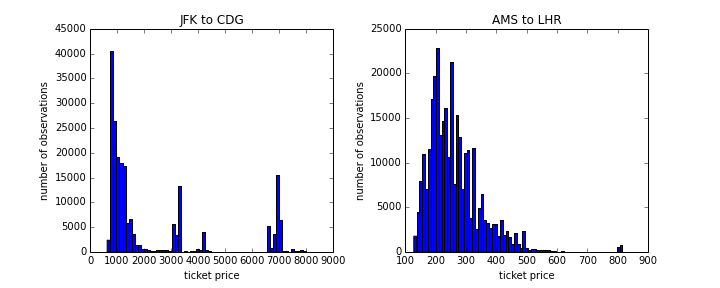
\includegraphics[width=.8\textwidth]{figures/Spread_JFK-CDG}
\caption{Spread of ticket prices}
\label{fig:SpreadOfTicketPrices}
\end{figure*}


The high range observed in the price fluctuations in some cases can also be assigned to sudden fare increases and drops. The high drops appearing at a single day before departure when the flight is yet to be sold out. This as a last resort of the airline to fill the seats on the plane. The high increases can be explained due to sold outs of economy~class tickets, which results in the display of first and business~class tickets.

For a better understanding of the price movements of airfares, one can look at the run sequence plot in \autoref{fig:4-plot}. The chart shows the average and standard deviation of price fluctuations of all the flights in the complete dataset. Instead of categorisation per route, the plot shows the statistics relative to its number of days before departure. One can clearly see that the mean fares for tickets are relatively stable for about the first three weeks of the analysis. The last three weeks up till departure there can clearly be seen significant and increasing price jumps at around 21~days, 14~days, 7~days, and the last few days before the flight. Furthermore, throughout the whole time frame, the volatility of the price fluctuations seems to be increasing.


\begin{figure*}
\centering
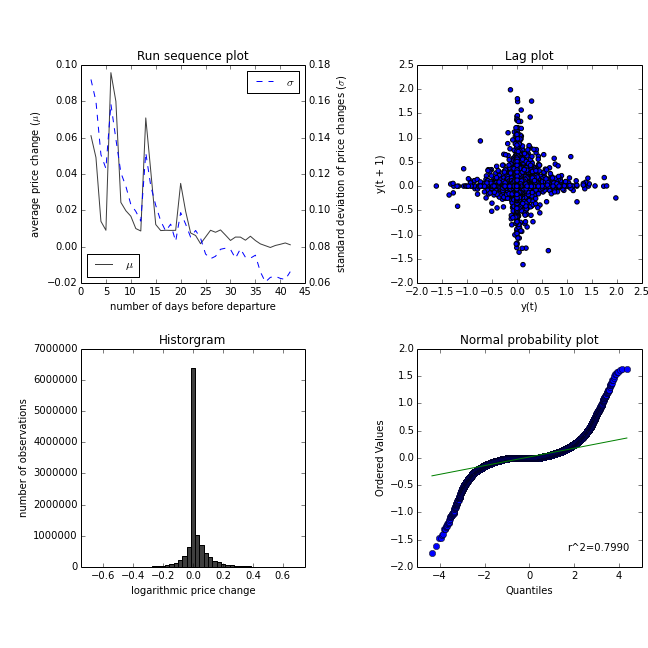
\includegraphics[width=.8\textwidth]{figures/4-plot}
\caption{4-Plot of the daily price fluctuations}
\label{fig:4-plot}
\end{figure*}


Due to these price jumps and increasing volatility, there will be more uncertainty on price fluctuations when nearing the departure date of the flight. Therefore it is expected that the option valuation models will yield higher airfare~lock-in prices for days closer to the flight's take-off. The higher standard deviation also creates more risk, which will likely result in higher losses and lower profits for those options than the ones that are offered at the beginning of the booking period.

The empirical distribution of all the ticket price fluctuations is presented in the histogram of \autoref{fig:4-plot}. The chart seems to display a normal distribution with a very high kurtosis and a strong tendency to the price change of 1. The \emph{one} can be interpreted as `no price change', and accounts for more than 56~percent --- or more than 6~million --- of all observed price changes. Due to this extreme peak, the empirical distribution can not be classified as a normally distributed one.

Analysis of the lag~plot in the same figure also results in the conclusion that the data on price fluctuations is not normally distributed. The plot consists of a random sample of 10,000~price changes, and clearly shows two lines in the figure near the 1-axes. Furthermore, the observations seem to be skewed to the positive quadrant of the figure. Both observations thus imply that the data is not random normally distributed.

The lag~plot also shows some outliers. However, as explained in \typenameref{subsec:outlierAnalysis}, these extreme values will be left included in the simulation models and data analysis. This is because these observations are valid empirical price changes, and could thereby happen in a real world setting.

The last visual confirmation that the data containing airfare fluctuations in not normally distributed can be found in the normal probability plot. This figure evidently shows that the data do not follow a straight line as a normal dataset would. 

The analysis of the 4~plot thus shows that the daily price fluctuations are not normally distributed. This is also confirmed by other normality tests. \autoref{tbl:NormalityTests} shows the results of the Shapiro--Wilk and Kolmogorov--Smirnov test for normality. Furthermore, it also displays the outcome of SciPy's implementation of \emph{normaltest}, which is based upon D'Agostino's K-squared and Pearon's chi-squared test.

All these statistical formula's test the null hypothesis, $H_0$, that the supplied sample came form a normally distributed population. As the outcomes of these tests show in the table, all of the tests lead to rejection of the null hypothesis. It can therefore be concluded that the daily price fluctuations do not follow a normally distributed curve.


\begin{table}
\centering
\begin{tabular}{l c c c}
\toprule
~  &  Test statistic  &  p-value  &  Reject $H_0$  \\
\midrule
Shapiro--Wilk test  &  0.66  &  $< 0.001$  & yes \\
Kolmogorov--Smirnov test  & 0.42  &  $< 0.001$  & yes \\
Normal test  & $6.34 \e{6}$  & $< 0.001$  & yes \\
\bottomrule
\end{tabular}
\caption{Tests for normality of daily returned values}
\label{tbl:NormalitTests}
\end{table}


The non-normality of the data implies that the changes in ticket prices are not completely random, and can therefore be predicted to some extend. Furthermore, because the daily changes are not normally distributed, the simulation model based upon Black--Scholes is not expected to perform well. This is due to one of the base assumptions of the Black-Scholes model which state that the underlying asset's returns follow a normal distribution. The optimal option price predictions according to this model are therefore likely to be far off of the optimal, which will lead to lower profits.

\subsection{Comparison of the training and test dataset}
This section compares the two different datasets with each other. As stated before, the first 4~weeks of data collected are assigned to the training (i.e., historical) dataset, and the last 2~weeks of the collection period to the test dataset. The two practically feasible option valuation methods in this research both use the historical set to make predictions of the price fluctuations in the test set. The Black--Scholes model uses the training dataset to determine the expected volatility of the ticket prices. The Monte~Carlo model bases its forecasts of airfares upon the empirical distribution seen in the same historical dataset. For these reasons, when the datasets differ from each other, the predictions of the models are likely to have a bigger error. The forecasts of the ticket prices then thus lie further from the actual observed values, which would lead to suboptimal option prices.

To compare the two distinct sets with each other, two statistical tests have been performed on the price fluctuations. The independent samples t-test assumes normally distributed samples, and could yield non-robust results if this is not the case. Because the daily price changes in this research do not seem to be normally distributed, I have chose to use the Kolmogorov--Smirnov two sample, and Mann--Whitney U tests. Both methods test the null hypothesis, $H_0$, that the supplied samples came from the same distribution.  The outcomes of both statistical methods can be found in \autoref{tbl:ComparisionOfDatasets}. A distinction is made between \emph{Individual} and \emph{Mean} observations. In the first category all the price observations were included in the dataset. For the latter case, the means of these price fluctuations were computed per day before departure and inserted into the set.


\begin{table}
\centering
\begin{tabular}{l l l r}
\toprule
~  &  ~  &  Test statistic  &  p-value  \\
\midrule
Individual  &   Kolmogorov--Smirnov test  & $0.07$  &  $< 0.001$  \\
~           &   Mann--Whitney U test  &  $2.23 \e{11}$ &  $< 0.001$ \\
Mean        &   Kolmogorov--Smirnov test  & $0.20$  &  $0.38$  \\
~           &   Mann--Whitney U test  &  $788$  &  $0.31$ \\
\bottomrule
\end{tabular}
\caption{Comparison of training and test dataset}
\label{tbl:ComparisionOfDatasets}
\end{table}


The results in the \emph{Individual} rows clearly show that it is very unlikely that both sets of single price changes are from the same population distribution. Both tests state that the null hypothesis can be rejected at an $\alpha$ of 0.001. While it was not expected that daily price fluctuations of the training and test set would differ, a explanation can be found in the data selection for both datasets. In this research, the flights for both sets were not randomly sampled, but rather selected based upon the departure date of the plane. This manner of data selection is chosen because it represents a valid real world case. When one would apply random sampling to establish two sets, a single set would consist of historical as well as `future' flights. Practically, however, this is not feasible, and an option selling company will only be able to collect historical prices and base its forecast on this set. The same logic is applied to this research, in which there is made a clear distinction between the two sets.

The possible explanation for the difference amongst the sets can thus be related to the fact that distinction is based upon a feature of the flight (i.e., departure date). It is therefore likely that the two datasets are dissimilar due to seasonality. A collection of more data over a longer period of time might void these problems.

While the statistical tests clearly show that the training and test dataset on individual price fluctuations differ from each other, the sets with means per day before departure show a significant similarity when $\alpha = 0.05$. A visual inspection also might lead to this conclusion. \autoref{fig:DailyPriceChangesBothSets} shows the average daily price changes relative to their number of days before departure for each set. Both lines seem to be overlapping.


\begin{figure*}
\centering
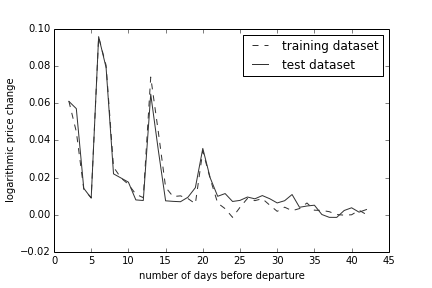
\includegraphics[width=.8\textwidth]{figures/Train-Test_DailyReturns}
\caption{Daily price changes of both datasets}
\label{fig:DailyPriceChangesBothSets}
\end{figure*}


Because this research will use the averages of the fluctuations to make its predictions in the empirical models, it is not expected that the difference amongst the sets in the individual cases will have a negative impact on the forecasting accuracy of the simulations. The similarities between the sets on an average level, however, are expected to have a positive impact on the results of the simulation models.

\autoref{tbl:StatisicalComparison} in \autoref{app:StatisticalComparisonDatasets} shows the same tests on a route level. Most of the routes show that both the price fluctuations in the training and test set come from the same distribution with a high probability. These flights are expected to perform well in the practical simulation models, as these make their forecasts of the test data by using the data in the training set. For some routes, however, there seems to be a significant difference amongst both sets. These routes include DFW to SFO, JFK to LHR, LAX to LAS, LAX to SFO, LHR to JFK, and LHR to LAX. These routes are expected to perform less in the simulation models based upon Black--Scholes and Monte-Carlo, as their historical input data does not align the observed price fluctuations.



\chapter{Results}
This part of the Master's Thesis will run the simulation models and compare the results of different option valuation methods. Furthermore, a sensitivity analysis will be performed to determine the influence of some of the parameters used in the models.

Due to the large amount of routes, only interesting or surprising results will be displayed and analysed in this chapter. Full tables with results can be found in the appendices \todo{ref}.


\section{Simulation 1: seller with perfect information and advance purchasing}
First, the simulation will be configuration to simulate the  seller with perfect information and the ability to purchase tickets in advance (i.e., long selling). The specific arrangement and description of its parameters can be found in \typenameref{chap:ModelDevelopment}. A summary of the level of the parameters can be found in \autoref{tbl:ParameterConfigAllKnowingSeller}.


\begin{table}
\begin{center}
\begin{tabular}{l l c r}
    \toprule
    \#  & Parameter  &  Symbol  &  Level \\
    \midrule
    1  &  option's days till maturity  &  $m$  & 3~days \\
    2  &  option's strike price  &  $p_S$  &  $p_I$  \\
    3  &  passenger's likelihood of travelling  &  $P^f$  &  U(0,1) \\
    4  &  passenger's expected increase airfare  &  $E_{p_t}$  &  6.55\,\% \\
    5  &  passenger's overestimation factor &  $\mbox{OEF}$  &  100\,\% \\
    6  &  arrival rate of passengers  &  ~  &  $(42 - m)$ per flight \\
    7  &  simulation's number of trials  &  $N$  &  150 \\
    \bottomrule
\end{tabular}
\caption{Parameters for the all knowing seller with foreknowledge}
\label{tbl:ParameterConfigAllKnowingSeller}
\end{center}
\end{table}


Next to the parameters of the simulation model, four assumptions have being made about the option seller, namely:
\begin{compactenum}
\item the seller knows the exact price movements of tickets (i.e., foreknowledge);
\item the seller knows the exact level of the customer's Willingness to Pay;
\item the seller knows in advance whether the customer will exercise its option;
\item the seller will buy tickets in advance when he knows the passenger will fly and the airfare increases.
\end{compactenum}

\vspace{1em}

The combination of these four assumptions characterize the all knowing option seller with foreknowledge. Due to these features, the option seller will be able to set the prices of options at the most optimal level. This will result in the highest level of profits a seller can ever gain from selling airfare~lock-in products in this setting.

This first simulation model will create an understanding on these maximum profits and optimal level of sales for the dataset. Furthermore, because uncertainties and risks of unavailable information have been eliminated, sensitivity analysis will also be performed. This sensitivity analysis will shed light on the influence of some of the parameters used in this section.


\subsection{Profitability of the model}
\label{subsec:ProfitabilityOfModel}
During the simulation, statistics on several properties will be collected. These properties allow the reader to get insight into the performance of the models. However, due to differences amongst the routes in terms of number of collected flights and height of ticket prices, comparison of performance between different outbound/inbound pairs is more difficult. Therefore, a ratio is introduced in this research, which enables better analysis between models and flight. The value is computed by multiplying the mean relative profits per option by the total percentage accepted, or:
$$\Pi_M = \Pi_O \times q$$

Where $\Pi_M$ is the profitability of the model, $\Pi_O$ denotes the profitability of an option, and $q$ represents the total number of options accepted by the passengers. The former two of these variables are in percentages relative to the mean ticket price, $\mu_{p_t}$, while the number of options accepted is the percentage of total generated customers.

This metric thus shows the expected profits as a percentage of the ticket price for every customer that requests an offer for an option. For example, consider a simulation model with 10,000 generated passengers. Of these customer's, 5,000 retrieve an offer at a level that they accept. After completion of the run, the model calculates that on average an accepted option yields 2\,\% of the ticket price as a profit. The profitability of the model thus is $0.02 \times 0.50 = 1\,\%$ profits per incoming customer. One can interpreted this as that for every possible customer that arrives in the model, the option seller is expected to gain 1\,\% of the ticket price in profits.

Because the measurement consists of only relative numbers, it can be used to compare outcomes of flights with a different number of generated passengers or ticket prices. This variable will thus be used throughout the rest of the model to compare distinct routes with each other.


\subsection{Analysis of the results}
\label{subsec:AnalysisPerfectInformation}
The simulation was first run on all the different routes using the parameters defined in previous section. The aggregated results for all routes can be found in \autoref{tbl:resultsAllKnowing}.


\begin{table}
\begin{center}
\begin{tabular}{c c | c c | c | c }
\toprule
    \multicolumn{2}{c|}{$\mu_{p_O}$} & \multicolumn{2}{c|}{$\Pi_O$}  &  $q$  & $\Pi_M$ \\[.4ex]
    \$  & \%  &  \$  & \%  & \%  & \% \\
    \midrule
16.50  &    3.28  &   16.50   &    3.28  &   100  &   3.28 \\
    \bottomrule
\end{tabular}
\caption{Simulation results of all knowing seller}
\label{tbl:resultsAllKnowing}
\end{center}
\end{table}


The columns labelled with $\mu_{p_O}$ contain the mean price of the option. The first column denoted the numeric value, while the second one gives the number in percentages relative to the mean ticket price. $\Pi_O$ denotes the profits gained per accepted option, and $q$ the percentage of options accepted. Lastly, $\Pi_M$ is the profitability of the model as described in \autoref{subsec:ProfitabilityOfModel}.

The outcomes of the model are in alignment with the expectations. The optimal option price on average is 3.28\,\% of the current ticket price, which is exactly half of the expected increase according to the passenger (6.55\,\%). This can be explained by the fact that the customer is willing to pay this expected increase multiplied by his likelihood of flying, $P^f$. Because the probability of flying is randomly drawn from an uniform distribution, the average of $P^f$ is $0.5$. Hence the average option price of 3.38\,\%. This was the case for every individual route in the simulation.

As also is shown in the table, the average profits gained for every accepted option -- $\Pi_O$ -- are equal to the average option price $\mu_{p_O}$. This is because of the fact that the seller has perfect information and is allowed to purchase tickets in advance. In this simulation, the option writer can make sure to buy the tickets at no price higher than the strike price, $p_S$. This is illustrated by the option seller's decision tree in \autoref{fig:PerfectInformationTree}. Because the seller has perfect information and makes his forecasts with 100~percent accuracy, he can purchase the tickets at the right time.

In the first case where the seller knows the passenger will never exercise the option, he will not undertake any action. The price the customer paid for the airfare~lock-in product is in its entirety profits to the seller.

The other cases represent passengers that will exercise their options on the date of maturity. When the price of the underlying ticket does \emph{not} increase, the seller is able to wait with the purchasing of the flight until maturity. However, when the airfare \emph{does} increase, the writer will be able to purchase the ticket in advance at the lower rate. Because of his foreknowledge, he does indeed have the information to choose the best time for buying a flight.

\insertfigure{PerfectInformationTree}{Decision tree of the all knowing seller with foreknowledge}

Because the option seller is always able to buy tickets for a flight at the lowest possible costs (i.e., at no level higher than $p_S$), he is also able to always offer an option to every passenger that has a request. This is represented by the $q$ of 100~percent in the table.

The profitability of the model in this case is also 3.28\,\%, the same as the average percentage of profits per airfare~lock-in product. This is explained by the $q$ of 100~percent. The profitability of the model thus shows that for every passenger that requests an option price in the simulation, the option seller is expected to gain 3.28\,\% of the ticket price in profits. This is the absolute maximum case in this configuration and will thus be used to compare other models with. 


\subsection{Sensitivity analysis}
After the first simulation, a sensitivity analysis was performed. The influence of the variables that were used to calculate the customer's Willingness To Pay were altered to determine their influence on the outcomes of the model.

The results of the effect of changes in the parameters were as could be theoretically expected. When a customer overestimated the expected increase in airfare by a single percent point, his Willingness To Pay increased with half a percent point. When the $\mbox{OEF}$ of a passenger decreased by a certain amount, the WTP would also decrease by half of that amount. 

$$ \Delta{\mbox{OEF}} = 0.5 \times \Delta{\mbox{WTP}} $$

This linear relation is easily explained by the fact that the customer's Willingness To Pay is closely related to his $P^f$. Because the average probability of flying is 0.5, every percentage increase results in a half percent increase of the WTP. Because in this first simulation it is assumed that the seller knows the exact level of the customer's WTP, the selling price of the airfare~lock-in product will automatically increase.

The same effect can be seen when increasing the number of days till maturity. After running the simulation, all of the expected outcomes were half of the passenger's expected increase in airfares.


\section{Simulation 2: seller with perfect information but without advance purchasing}
The second simulation will be based upon the previous run, but drops a single assumption. This model will simulate an option seller with perfect information that does not have the possibility to purchase tickets in advance. He therefore will not be able to always purchase the tickets at the lowest price, and has to wait till maturity before he can buy the flight ticket when requested by the customer. However, this model still assumes that the option seller has the ability to make predictions with a 100~percent accuracy, and also does know whether the passenger will exercise his option on the date of maturity. The decision tree in \autoref{fig:NoAdvanceSellingTree} gives an overview of the decision process of the option seller that has no ability of buying the tickets in advance.

\insertfigure{NoAdvanceSellingTree}{Decision tree of the all knowing seller with foreknowledge but no advance purchase}
 
As can be observed from the figure, the option seller will only offer an option product to the passenger when he either knows the customer will not exercise the option, or when the future ticket price is lower than the strike price plus the Willingness To Pay of the consumer. Because in this simulation the strike price, $p_S$ is always equal to the initially observed airfare, $p_I$, the latter case can also be described as when the price increase of an option is less than the price of the customers WTP.




\begin{table}
\begin{center}
\begin{tabular}{c c | c c | c c | c | c }
\toprule
\multicolumn{2}{c|}{Airport}  &  \multicolumn{2}{c|}{$\mu_{p_O}$} & \multicolumn{2}{c|}{$\Pi_O$}  &  $q$  & $\Pi_M$ \\[.4ex]
from  &  to  &  \$  & \%  &  \$  & \%  & \%  & \% \\
    \midrule
AMS  &  CDG  &    6.48  &  2.97  &    6.16  &  2.83  &  76.59  &  2.17 \\
~    &  DXB  &   18.38  &  3.16  &   18.24  &  3.14  &  90.11  &  2.83 \\
~    &  JFK  &   25.61  &  3.11  &   23.81  &  2.88  &  83.90  &  2.41 \\
~    &  LHR  &    7.93  &  3.07  &    7.36  &  2.84  &  81.05  &  2.31 \\[.5ex]
ATL  &  LAX  &   11.58  &  3.06  &   10.57  &  2.78  &  80.13  &  2.23 \\
~    &  MCO  &    7.23  &  2.96  &    6.81  &  2.80  &  75.90  &  2.12 \\[.5ex]
CDG  &  AMS  &    6.90  &  2.99  &    6.58  &  2.86  &  77.59  &  2.22 \\
~    &  LHR  &    6.68  &  3.08  &    6.26  &  2.88  &  82.17  &  2.37 \\[.5ex]
DEN  &  FLL  &    5.61  &  3.12  &    5.29  &  2.96  &  84.39  &  2.50 \\
~    &  PHX  &    5.55  &  3.08  &    5.09  &  2.82  &  81.40  &  2.29 \\[.5ex]
DFW  &  LAX  &    8.67  &  3.03  &    8.13  &  2.84  &  79.82  &  2.27 \\
~    &  SFO  &   11.32  &  3.02  &   10.59  &  2.82  &  78.67  &  2.21 \\[.5ex]
JFK  &  CDG  &   89.64  &  3.16  &   86.05  &  2.96  &  87.94  &  2.61 \\
~    &  LHR  &   30.24  &  3.17  &   27.97  &  2.90  &  87.82  &  2.55 \\[.5ex]
LAX  &  LAS  &    6.48  &  3.08  &    6.08  &  2.88  &  82.59  &  2.38 \\
~    &  SFO  &    6.81  &  3.03  &    6.39  &  2.84  &  79.39  &  2.26 \\[.5ex]
LHR  &  AMS  &    7.32  &  3.06  &    6.71  &  2.80  &  80.22  &  2.25 \\
~    &  JFK  &   27.79  &  3.23  &   25.51  &  2.93  &  91.94  &  2.69 \\
~    &  LAX  &   41.55  &  3.22  &   38.19  &  2.90  &  90.62  &  2.63 \\
~    &  MAD  &    8.37  &  3.07  &    7.82  &  2.87  &  82.03  &  2.36 \\[.5ex]
ORD  &  BOS  &    7.46  &  3.06  &    6.80  &  2.77  &  79.90  &  2.22 \\
~    &  LGA  &    8.33  &  3.12  &    7.73  &  2.88  &  84.19  &  2.43 \\
\midrule
Means &  ~   &   16.18  &  3.08  &   15.19  &  2.87  &  82.65  &  2.38 \\
    \bottomrule
\end{tabular}
\caption{Simulation results of all knowing seller without advance purchasing}
\label{tbl:resultsSecond}
\end{center}
\end{table}




%%  Backmatter
\appendix
\chapter{Data extracted from Google Flight's RPC-request}
\label{app:DataExtractedFromGoogleFlightsRPCRequest}
\begin{table}[h]
	\centering
    \begin{tabular}{l l}
        \toprule
        Index                         & Description                                                              \\
        \midrule
        Array[0][0][1][3][0][*] 	  & Array of all possible segments (Segment)                                 \\ 
        Array[0][0][1][3][1][*] 	  & Array of all possible routes (Route)                                     \\ 
        Segment[1][0]                 & Departure airport (IATA code)                                            \\ 
        Segment[1][1]                 & Departure date and time                                                  \\ 
        Segment[1][2]                 & Arrival airport (IATA code)                                              \\ 
        Segment[1][3]                 & Arrival date and time                                                    \\ 
        Segment[1][4]                 & Carrier code (IATA code)                                                 \\ 
        Segment[1][5]                 & Flight number                                                            \\ 
        Route[0][0]                   & Index of outbound segments                                               \\ 
        Route[0][1]                   & Index of inbound segments                                                \\ 
        Route[1]                      & Price of round-trip                                                      \\ 
        Route[3][0][0]                & Ticketing code of outbound flight (IATA code) \\ 
        Route[3][1][0]                & Ticketing code of inbound flight (IATA code) \\
    \bottomrule
    \end{tabular}
	\caption{Information in Google Flight's RPC response}
\end{table}



\chapter{Selected routes}
\label{app:SelectedRoutes}
\begin{table}[h]
	\centering
    \begin{tabular}{ l l l l }
        \toprule
        ~           & Airports & ~ \\
        \cmidrule{2-4}
        Category        & Outbound & Inbound        \\ 
        \midrule
        US Domestic & ATL & MCO & LAX \\
        ~           & DEN & PHX & FLL \\
        ~           & DFW & LAX & SFO \\
        ~           & LAX & SFO & LAS \\
        ~           & ORD & LGA & BOS \\
        EU Domestic & AMS & CDG & LHR \\
		~           & CDG & AMS & LHR \\
		~           & LHR & AMS & MAD \\
        International & AMS & DXB & JFK \\ 
        ~             & JFK & CDG & LHR \\
        ~             & LHR & JFK & LAX \\
        \bottomrule
    \end{tabular}
	\caption{Routes to be examined}
\end{table}



\chapter{Sample JSON RPC}
\label{app:SampleJSONRPC}
\small
\begin{verbatim}
{'1': [{'1': 'fs', '2':
  '{"1":{"1":[
    {"1":[ATL],          # departure airport
     "2":[MCO],          # arrival airport
     "3":"2013-08-26"},  # departure date
    {"1":[MCO],          # departure airport return
     "2":[ATL},          # arrival airport return
     "3":"2013-08-19"}   # departure date return
  ]}}', u'4': 1}],
'2': {'1': [{'1': 'b_am', '2': 'fs'},
            {'1': 'b_qu', '2': '2'},
            {'1': 'b_qc', '2': '2'}
]}}
\end{verbatim}



\chapter{Adapted Black-Scholes formula}
\label{app:AdaptedBlackScholesFormula}
\begin{align*}
p_O &= p_I \times N(d_1) - p_S \times e^{-rT}N(d_2) \\
d_1 &= \frac{\ln(p_I/p_S) + (r + \sigma^2/2)T}{\sigma \sqrt{T}} \\
d_2 &= d_1 - \sigma \sqrt{T}
\end{align*}

\begin{compactdesc}
\item[$p_O$] is the call value
\item[$p_I$] is the initial price of the flight
\item[$T$] is the time to maturity
\item[$N(\cdot)$] is the cumulative normal probability
\item[$\sigma$] is the volatility of returns of the underlying flight
\item[$p_S$] is the strike price of the option
\item[$r$] is the risk free rate
\vspace{1ex}
\end{compactdesc}



\chapter{Simulation results of all knowing seller}
\label{app:SimulationResultsAllKnowingSeller}
The table below gives the results of the simulation of the all knowing seller with foresight. An analysis of the results can be found in \autoref{subsec:AnalysisOfAllKnowing}.
\\[2em]
\begin{table}[h]
    \begin{center}
        \begin{tabular}{l r c c c c c c}
            \toprule
            \multicolumn{2}{c}{Airport}  &  Ticket & \multicolumn{2}{c}{Option price} & \multicolumn{2}{c}{Options profits}  &  Sold  \\[.4ex]
            from  &  to  &  \$   &  \$  & \%  &  \$  & \%  & \%  \\
            \midrule
AMS  &  CDG  &     226  &    8.93  &   3.95  &    8.60  &   96.30  &   75.94 \\
~    &  DXB  &     591  &   23.18  &   3.92  &   21.78  &   93.95  &   32.80 \\
~    &  JFK  &     852  &   18.15  &   2.13  &   17.46  &   96.19  &   72.51 \\
~    &  LHR  &     259  &    6.67  &   2.58  &    6.33  &   94.84  &   78.06 \\[.5ex]
ATL  &  LAX  &     394  &   12.23  &   3.11  &   11.59  &   94.73  &   70.28 \\
~    &  MCO  &     252  &   11.47  &   4.55  &   10.74  &   93.56  &   75.85 \\[.5ex]
CDG  &  AMS  &     240  &    8.56  &   3.57  &    8.26  &   96.43  &   76.84 \\
~    &  LHR  &     221  &    4.68  &   2.11  &    4.54  &   97.12  &   78.95 \\[.5ex]
DEN  &  FLL  &     182  &    8.68  &   4.76  &    8.10  &   93.26  &   60.43 \\
~    &  PHX  &     189  &    7.20  &   3.81  &    6.67  &   92.66  &   75.87 \\[.5ex]
DFW  &  LAX  &     313  &   17.63  &   5.63  &   16.01  &   90.84  &   56.91 \\
~    &  SFO  &     388  &   26.72  &   6.89  &   24.80  &   92.82  &   57.55 \\[.5ex]
JFK  &  CDG  &    2637  &  154.78  &   5.87  &  149.27  &   96.44  &   74.73 \\
~    &  LHR  &    1000  &   92.28  &   9.23  &   86.91  &   94.18  &   92.03 \\[.5ex]
LAX  &  LAS  &     212  &   11.02  &   5.20  &   10.25  &   92.97  &   75.41 \\
~    &  SFO  &     222  &   21.00  &   9.48  &   19.43  &   92.54  &   75.81 \\[.5ex]
LHR  &  AMS  &     242  &    6.46  &   2.67  &    6.05  &   93.60  &   77.59 \\
~    &  JFK  &     864  &   74.64  &   8.64  &   70.58  &   94.56  &   94.88 \\
~    &  LAX  &    1286  &  122.79  &   9.54  &  117.51  &   95.70  &   91.96 \\
~    &  MAD  &     282  &    5.00  &   1.77  &    4.76  &   95.24  &   79.04 \\[.5ex]
ORD  &  BOS  &     249  &   13.53  &   5.43  &   12.37  &   91.49  &   76.96 \\
~    &  LGA  &     273  &   13.13  &   4.81  &   12.09  &   92.03  &   74.46 \\
            \bottomrule
        \end{tabular}
        \caption{Simulation results of all knowing seller}
        \label{tbl:resultsAllKnowing}
    \end{center}
\end{table}


\chapter{Simulation results of Black--Scholes model}
\label{app:SimulationResultsBS}
The table below gives the results of the simulation of the Black--Scholes model. An analysis of the results can be found in \autoref{subsec:AnalysisOfBS}.
\\[2em]
\begin{table}[h]
    \begin{center}
        \begin{tabular}{l r c c c c c c}
            \toprule
            \multicolumn{2}{c}{Airport}  &  Ticket & \multicolumn{2}{c}{Option price} & \multicolumn{2}{c}{Options profits}  &  Sold  \\[.4ex]
            from  &  to  &  \$   &  \$  & \%  &  \$  & \%  & \%  \\
            \midrule
AMS  &  CDG  &     226  &   23.32  &  10.32  &   -1.74  &   -7.46  &   53.85 \\
~    &  DXB  &     591  &   89.97  &  15.23  &   -9.81  &  -10.90  &   12.82 \\
~    &  JFK  &     852  &   78.93  &   9.27  &  -41.16  &  -52.14  &   25.64 \\
~    &  LHR  &     259  &   18.00  &   6.96  &   -0.55  &   -3.06  &   48.72 \\[.5ex]
ATL  &  LAX  &     394  &   39.80  &  10.11  &   -4.55  &  -11.44  &   35.90 \\
~    &  MCO  &     252  &   25.81  &  10.24  &    2.50  &    9.70  &   61.54 \\[.5ex]
CDG  &  AMS  &     240  &   23.86  &   9.95  &   -1.11  &   -4.63  &   51.28 \\
~    &  LHR  &     221  &   14.33  &   6.48  &   -3.02  &  -21.05  &   25.64 \\[.5ex]
DEN  &  FLL  &     182  &   23.42  &  12.85  &  -15.12  &  -64.55  &   25.64 \\
~    &  PHX  &     189  &   23.46  &  12.42  &    1.14  &    4.86  &   33.33 \\[.5ex]
DFW  &  LAX  &     313  &   47.61  &  15.21  &  -31.37  &  -65.90  &   33.33 \\
~    &  SFO  &     388  &   67.08  &  17.29  &  -38.55  &  -57.47  &   30.77 \\[.5ex]
JFK  &  CDG  &    2637  &  336.52  &  12.76  &  179.20  &   53.25  &   35.90 \\
~    &  LHR  &    1000  &  142.97  &  14.30  &   47.34  &   33.11  &   69.23 \\[.5ex]
LAX  &  LAS  &     212  &   32.13  &  15.15  &   -2.47  &   -7.68  &   35.90 \\
~    &  SFO  &     222  &   38.84  &  17.53  &   14.16  &   36.45  &   48.72 \\[.5ex]
LHR  &  AMS  &     242  &   18.37  &   7.60  &    0.28  &    1.51  &   43.59 \\
~    &  JFK  &     864  &  127.12  &  14.72  &   84.23  &   66.26  &   58.97 \\
~    &  LAX  &    1286  &  198.47  &  15.43  &   99.67  &   50.22  &   53.85 \\
~    &  MAD  &     282  &   22.49  &   7.96  &   -6.28  &  -27.95  &   20.51 \\[.5ex]
ORD  &  BOS  &     249  &   40.87  &  16.40  &  -12.36  &  -30.24  &   33.33 \\
~    &  LGA  &     273  &   38.28  &  14.02  &   -0.98  &   -2.57  &   38.46 \\
            \bottomrule
        \end{tabular}
        \caption{Simulation results of Black--Scholes model}
        \label{tbl:resultsBS}
    \end{center}
\end{table}

 %  before backmatter, because of chapter numbering
\backmatter
\bibliography{ThesisBiblio}
\bibliographystyle{apacite}

\end{document}
